\addtocounter{chapter}{0} % يضمن مزامنة الفهرس
\setcounter{figure}{0}    % يصفر عداد الأشكال لتبدأ من 1
\setcounter{table}{0}     % يصفر عداد الجداول لتبدأ من 1
\renewcommand{\thefigure}{6.\arabic{figure}} % يجبر اللاحقة تبدأ برقم 6
\renewcommand{\thetable}{6.\arabic{table}}   % يجبر الجداول تبدأ برقم 6
\section{Hardware Implementation of the Interleaved Boost Converter}

\subsection{Introduction to Hardware Design}
The generation stage of the solar-powered EV charging station relies entirely on an Interleaved Boost Converter topology. Hardware implementation of this specific power electronics block is critical for managing the stochastic electrical behavior of the photovoltaic (PV) source. Unlike conventional single-phase boost configurations, interleaving shifts parallel switching states by a deterministic phase angle.

This structural approach offers two vital advantages for our hardware setup:
\begin{enumerate}
    \item \textbf{Input Current Ripple Cancellation:} The destructive interference of the phase-shifted triangular inductor currents drastically smooths out the total current drawn from the PV panel, preventing premature cellular degradation.
    \item \textbf{Thermal and Component Stress Distribution:} The total power flow is split evenly between two independent tracking paths. This cuts conduction losses, minimizes core saturation risks in the inductors, and permits the utilization of power MOSFETs with lower continuous current ratings.
\end{enumerate}
\begin{figure}[H]
    \centering
    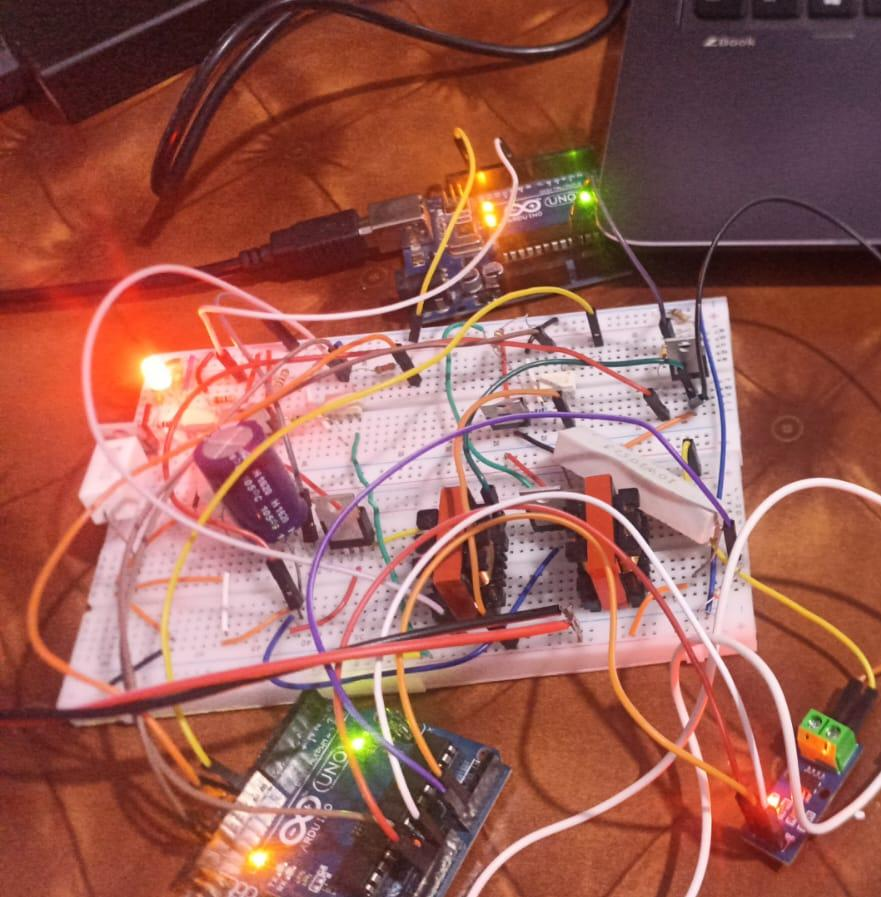
\includegraphics[width=0.8\textwidth]{Figures/kk.jpeg} % Place your hardware schematic here
    \caption{First prototype of the two-phase Interleaved Boost Converter.}
    \label{fig:interleaved_hardware_schematic}
\end{figure}
\begin{figure}[H]
    \centering
    \includegraphics[width=0.8\textwidth]{Figures/interleaved_hardware_schematic.png} % Place your hardware schematic here
    \caption{Complete hardware power stage schematic of the two-phase Interleaved Boost Converter.}
    \label{fig:interleaved_hardware_schematic}
\end{figure}

\subsection{Open-Loop Characterization}
The initial phase of hardware commissioning involves open-loop verification. In this configuration, the feedback loops are entirely disconnected, and the switching devices receive a static, predefined duty cycle ($D$) generated by an external signal source or a microcontroller timer peripheral. 

The primary objective of open-loop testing is to validate the structural integrity of the power stage layout, verify the 180$^\circ$ phase shift between the gate drivers, and map the absolute physical output voltage ($V_{out}$) against the continuous mathematical ideal:
\begin{equation}
    V_{out} = \frac{V_{in}}{1 - D}
\end{equation}

During this operational state, because there is no active correction mechanism, the output voltage remains highly sensitive to input perturbations and load fluctuations. If the input PV voltage sags due to changing ambient conditions or if the equivalent load resistance drops, the output voltage naturally drops as well.

Assuming input voltage is 12V and $Rth = 10\ \Omega$., below are the output voltages at some duties, where the load is $100\ \Omega$

\begin{figure}[H]
    \centering
    % --- الصورة الأولى (اليسار) ---
    \begin{subfigure}[b]{0.48\textwidth}
        \centering
        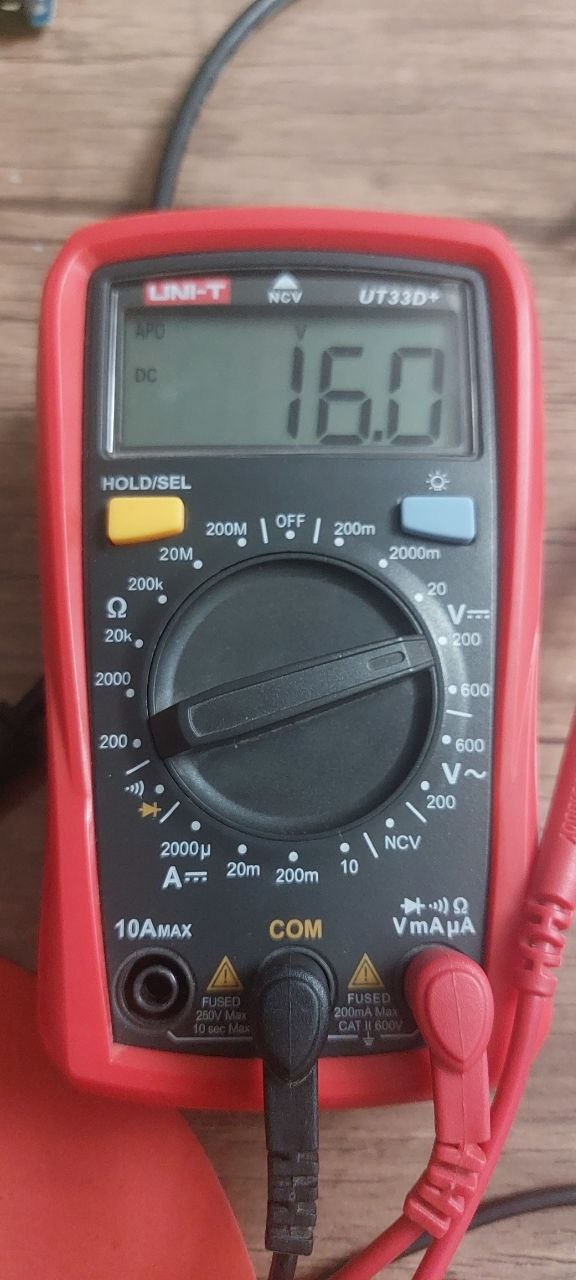
\includegraphics[width=0.48\textwidth]{Figures/111.jpg}
        \caption{$V_{out}$ at $D = 0.5$}
        \label{fig:vout_d_05}
    \end{subfigure}
    \hfill % بيعمل مسافة أفقية مرنة عشان يوزع الصورتين على عرض الصفحة بالظبط
    % --- الصورة الثانية (اليمين) ---
    \begin{subfigure}[b]{0.48\textwidth}
        \centering
        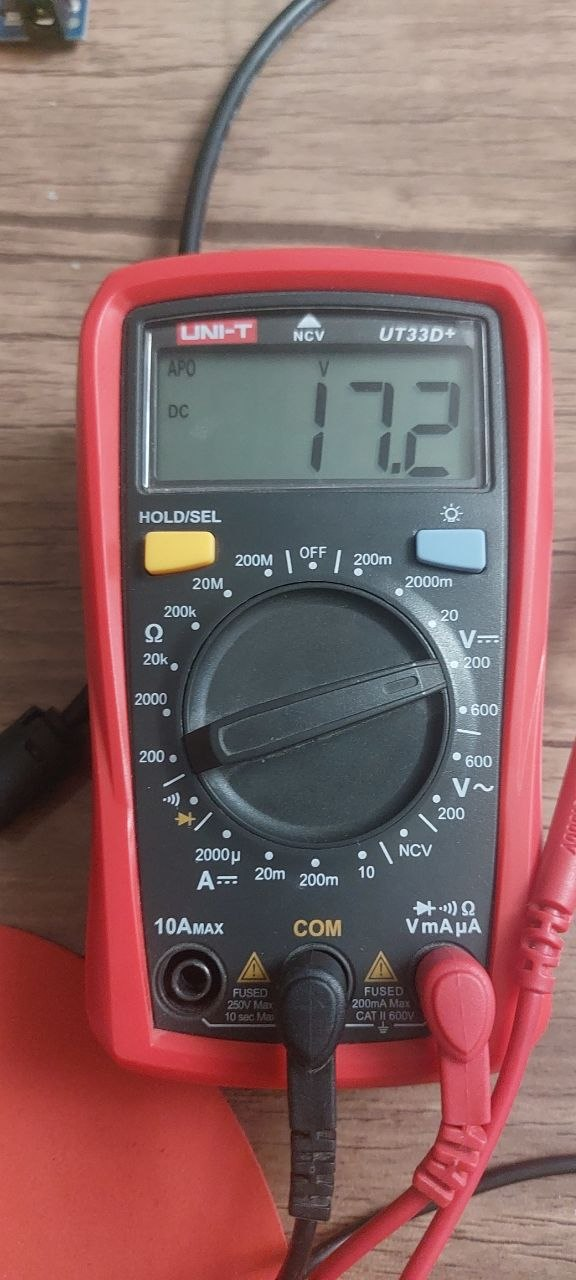
\includegraphics[width=0.48\textwidth]{Figures/222.jpg}
        \caption{$V_{out}$ at $D = 0.6$}
        \label{fig:vout_d_06}
    \end{subfigure}
    
    % --- الصورة الأولى (اليسار) ---
    \begin{subfigure}[b]{0.48\textwidth}
        \centering
        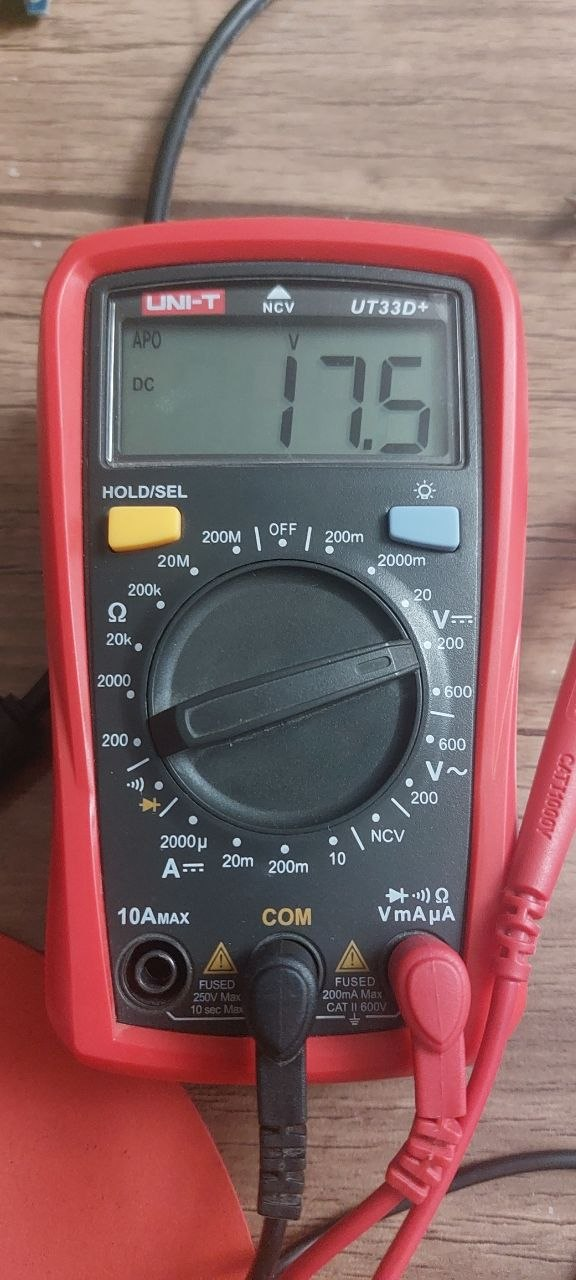
\includegraphics[width=0.48\textwidth]{Figures/333.jpg}
        \caption{$V_{out}$ at $D = 0.7$}
        \label{fig:vout_d_05}
    \end{subfigure}
    \hfill % بيعمل مسافة أفقية مرنة عشان يوزع الصورتين على عرض الصفحة بالظبط
    % --- الصورة الثانية (اليمين) ---
    \begin{subfigure}[b]{0.48\textwidth}
        \centering
        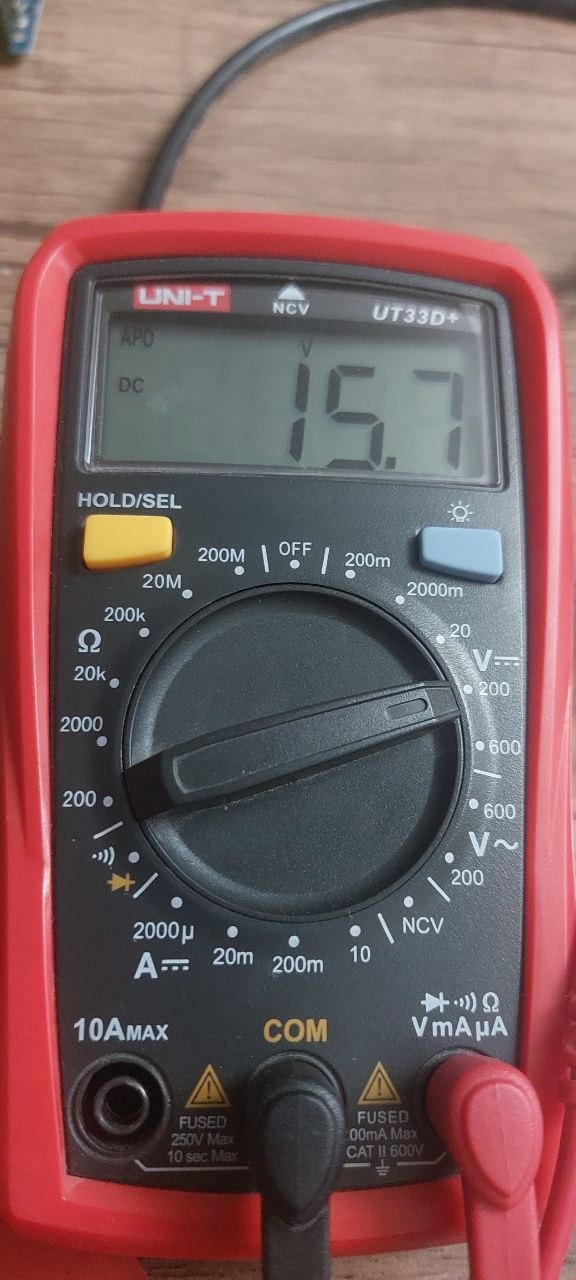
\includegraphics[width=0.48\textwidth]{Figures/444.jpg}
        \caption{$V_{out}$ at $D = 0.8$}
        \label{fig:vout_d_06}
    \end{subfigure}
    
    % --- الكابشن الرئيسي والمشترك للمجموعة ---
    \caption{Experimental output voltage ($V_{out}$) waveforms under different open-loop duty cycle conditions.}
    \label{fig:open_loop_waveforms_comparison}
\end{figure}

The empirical waveforms captured during this testing state illustrate the fixed-frequency pulse train. While the switching node pulses alternate properly, minor voltage sags and non-linearities are visible due to parasitic components such as the inductor ESR ($r_L$), capacitor ESR ($r_C$), and the forward voltage drop across the power diodes.

\begin{figure}[H]
    \centering
    % --- الصورة الأولى (اليسار) ---
    \begin{subfigure}[b]{0.48\textwidth}
        \centering
        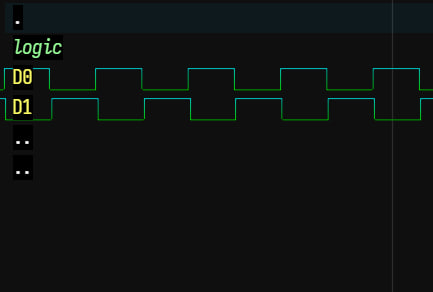
\includegraphics[width=0.78\textwidth]{Figures/1111.jpg}
        \caption{$D = 0.5$}
        \label{fig:vout_d_05}
    \end{subfigure}
    \hfill % بيعمل مسافة أفقية مرنة عشان يوزع الصورتين على عرض الصفحة بالظبط
    % --- الصورة الثانية (اليمين) ---
    \begin{subfigure}[b]{0.48\textwidth}
        \centering
        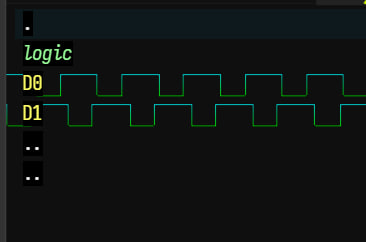
\includegraphics[width=0.78\textwidth]{Figures/2222.jpg}
        \caption{$D = 0.6$}
        \label{fig:vout_d_06}
    \end{subfigure}

    \begin{subfigure}[b]{0.48\textwidth}
        \centering
        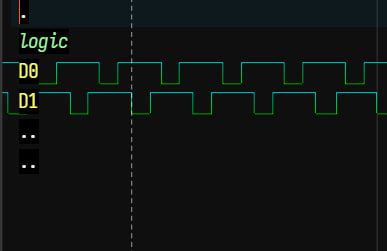
\includegraphics[width=0.78\textwidth]{Figures/3333.jpg}
        \caption{$D = 0.7$}
        \label{fig:vout_d_05}
    \end{subfigure}
    \hfill % بيعمل مسافة أفقية مرنة عشان يوزع الصورتين على عرض الصفحة بالظبط
    % --- الصورة الثانية (اليمين) ---
    \begin{subfigure}[b]{0.48\textwidth}
        \centering
        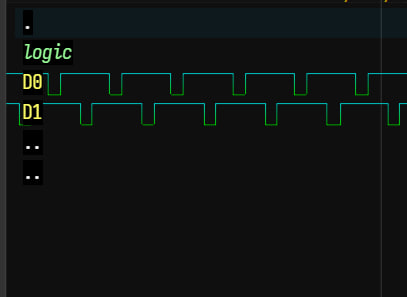
\includegraphics[width=0.78\textwidth]{Figures/4444.jpg}
        \caption{$D = 0.8$}
        \label{fig:vout_d_06}
    \end{subfigure}
    
    % --- الكابشن الرئيسي والمشترك للمجموعة ---
    \caption{Different waveforms for duties.}
    \label{fig:open_loop_waveforms_comparison}
\end{figure}

\subsection{Closed-Loop Hysteresis Voltage Control}
To mitigate the inherent voltage sagging characterized during open-loop testing and to guarantee a rock-solid, invariant intermediate bus for the subsequent charging converter stages, an active closed-loop hysteresis voltage control framework is implemented. This strategy completely replaces linear PID control controllers with a non-linear bang-bang regulation mechanism to achieve a higher dynamic bandwidth and instantaneous response to transient states.

The output voltage ($V_{out}$) from the bulk capacitor bank is downscaled via a high-precision voltage sensing divider network and fed directly into the analog-to-digital conversion interface of the control unit. This real-time tracking variable is continuously compared against the target reference index ($V_{ref} = 10\text{ V}$), deriving the instantaneous voltage loop tracking error:
\begin{equation}
    e_v(t) = V_{ref} - V_{out}(t)
\end{equation}

Instead of passing through linear compensators, the error signal is evaluated directly by a hysteresis comparator logic loop with a predefined tolerance error band ($\pm h$). The control rule governs the state of the interleaved gating signals according to the following direct switching logic:
\begin{align}
    \text{If } e_v(t) > +h &\implies \text{Increase Charging Duty Cycle (Boost Energy Flow)} \\
    \text{If } e_v(t) < -h &\implies \text{Decrease Charging Duty Cycle (Attenuate Voltage Rise)}
\end{align}

To rigorously evaluate the robust regulation performance of this hysteresis framework under transient load perturbations, an auxiliary load-switching sub-circuit was integrated into the hardware prototype.
\newpage
This setup consists of an electronically controlled switch connected in series with a physical $47\ \Omega$ load resistor, placed in parallel across the output terminal link. Rapidly toggling this switch creates step-load variations that force sudden current injections, testing the converter's transient settling speed.

\subsubsection{Input Voltage}
\begin{figure}[H]
    \centering
    \begin{subfigure}[b]{0.45\textwidth}
        \centering
        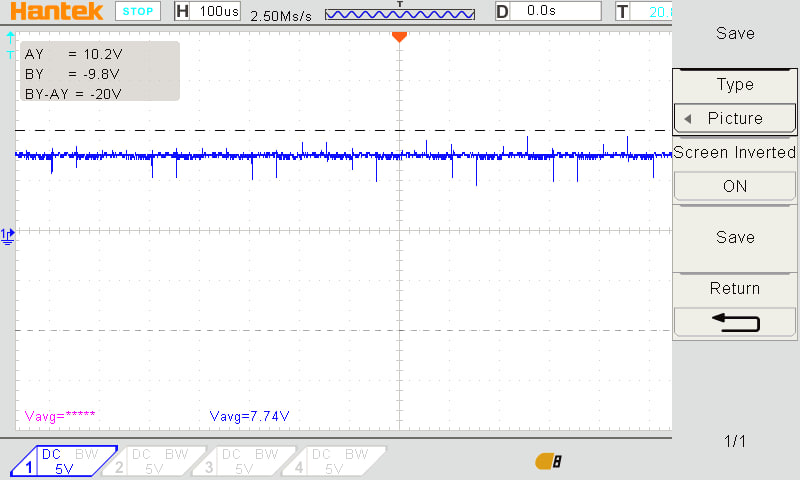
\includegraphics[width=\linewidth]{Figures/11111.jpg} % Place photo for first duty/load condition here
        \caption{$V_{in}$ at 0.5 duty.}
        \label{fig:hysteresis_v_d1}
    \end{subfigure}
    \hfill
    \begin{subfigure}[b]{0.45\textwidth}
        \centering
        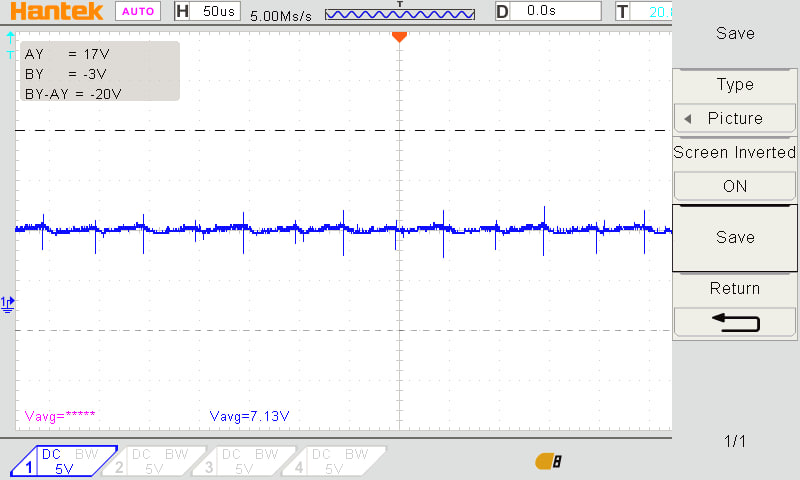
\includegraphics[width=\linewidth]{Figures/22222.jpg} % Place photo for second duty/load condition here
        \caption{$V_{in}$ at 0.6 duty.}
        \label{fig:hysteresis_v_d2}
    \end{subfigure}
    \label{fig:hysteresis_voltage_results}
    \centering
    \begin{subfigure}[b]{0.45\textwidth}
        \centering
        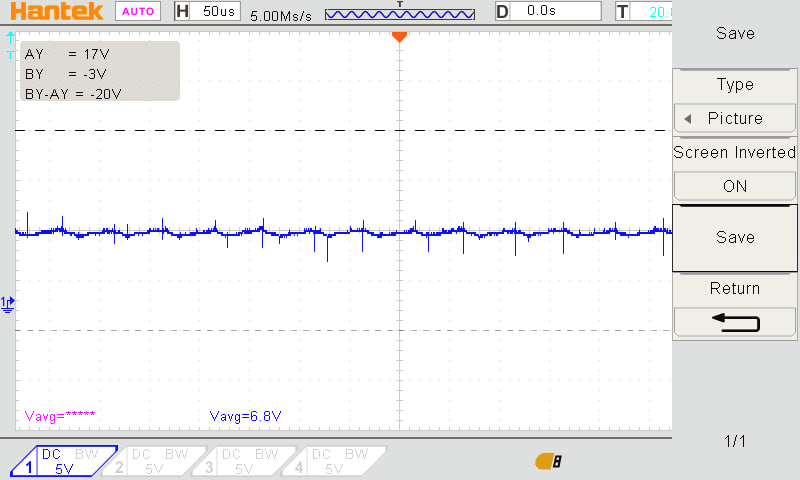
\includegraphics[width=\linewidth]{Figures/33333.jpg} % Place photo for first duty/load condition here
        \caption{$V_{in}$ at 0.65 duty.}
        \label{fig:hysteresis_v_d1}
    \end{subfigure}
    \hfill
    \begin{subfigure}[b]{0.45\textwidth}
        \centering
        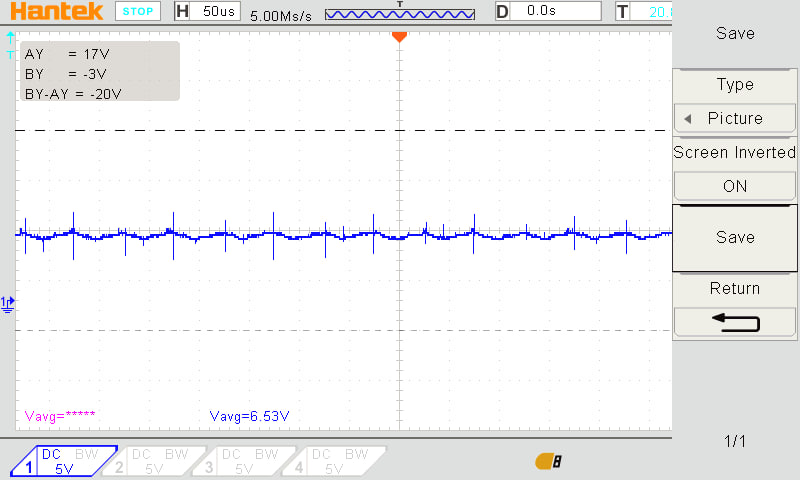
\includegraphics[width=\linewidth]{Figures/44444.jpg} % Place photo for second duty/load condition here
        \caption{$V_{in}$ at 0.7 duty.}
        \label{fig:hysteresis_v_d2}
    \end{subfigure}
    \label{fig:hysteresis_voltage_results}
    \centering
    \begin{subfigure}[b]{0.45\textwidth}
        \centering
        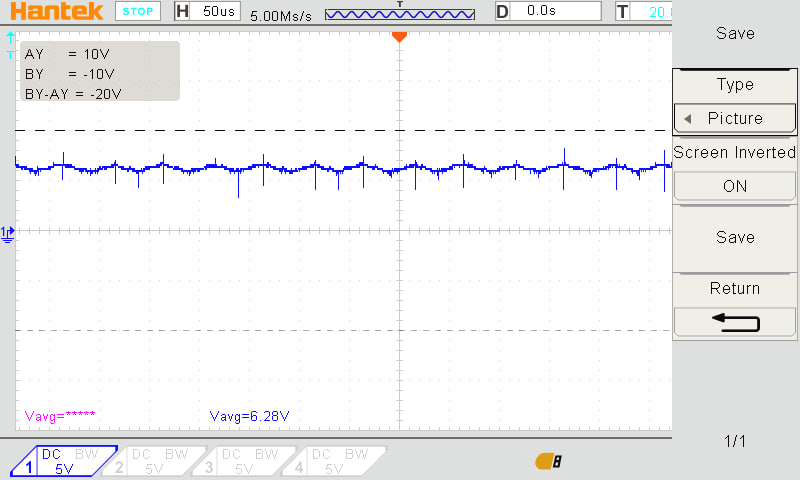
\includegraphics[width=\linewidth]{Figures/55555.jpg} % Place photo for first duty/load condition here
        \caption{$V_{in}$ at 0.75 duty.}
        \label{fig:hysteresis_v_d1}
    \end{subfigure}
    \hfill
    \begin{subfigure}[b]{0.45\textwidth}
        \centering
        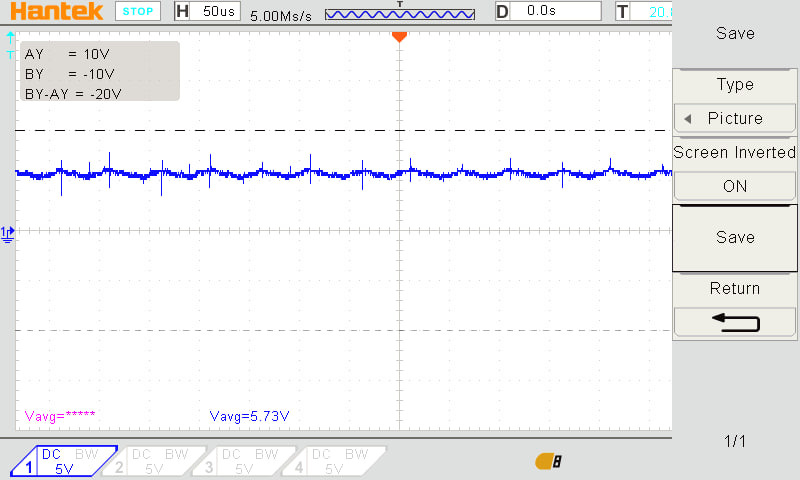
\includegraphics[width=\linewidth]{Figures/66666.jpg} % Place photo for second duty/load condition here
        \caption{$V_{in}$ at 0.8 duty.}
        \label{fig:hysteresis_v_d2}
    \end{subfigure}
    \label{fig:hysteresis_voltage_results}
    \centering
    \begin{subfigure}[b]{0.45\textwidth}
        \centering
        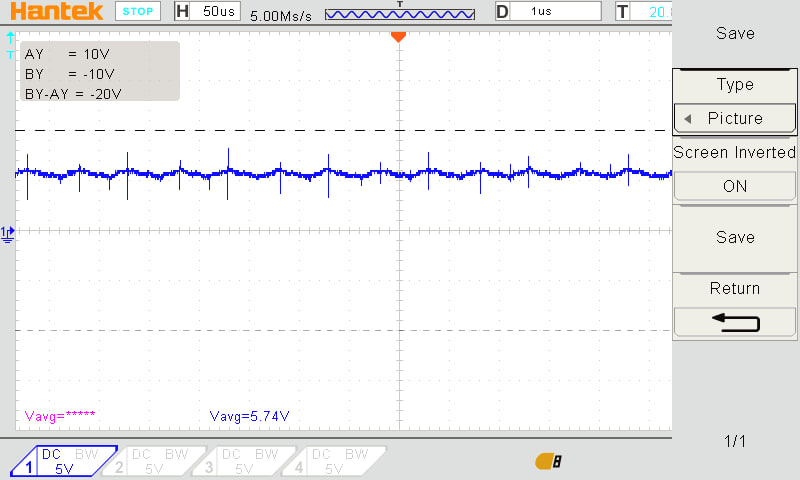
\includegraphics[width=\linewidth]{Figures/77777.jpg} % Place photo for first duty/load condition here
        \caption{$V_{in}$ at 0.82 duty.}
        \label{fig:hysteresis_v_d1}
    \end{subfigure}
    \hfill
    \begin{subfigure}[b]{0.45\textwidth}
        \centering
        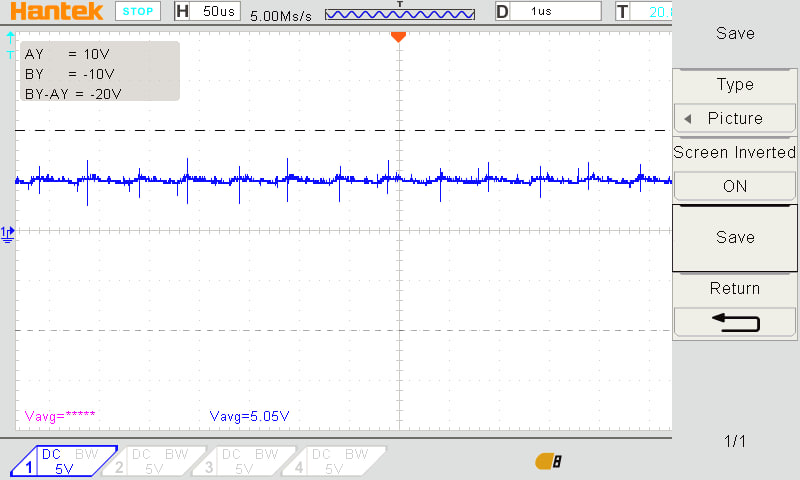
\includegraphics[width=\linewidth]{Figures/88888.jpg} % Place photo for second duty/load condition here
        \caption{$V_{in}$ at 0.9 duty.}
        \label{fig:hysteresis_v_d2}
    \end{subfigure}
    \caption{$V_{in}$ at different duties.}
    \label{fig:hysteresis_voltage_results}
\end{figure}
\newpage
\subsubsection{Output Voltage}
\begin{figure}[H]
    \centering
    \begin{subfigure}[b]{0.45\textwidth}
        \centering
        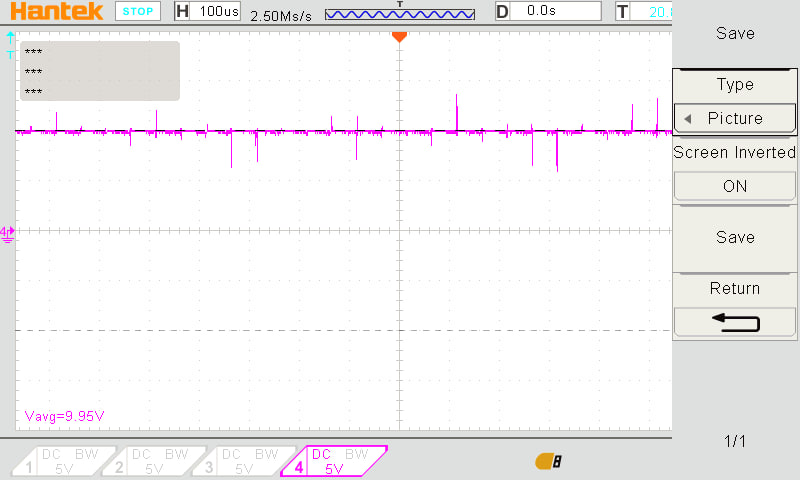
\includegraphics[width=\linewidth]{Figures/01.jpg} % Place photo for first duty/load condition here
        \caption{$V_{out}$ at 0.5 duty.}
        \label{fig:hysteresis_v_d1}
    \end{subfigure}
    \hfill
    \begin{subfigure}[b]{0.45\textwidth}
        \centering
        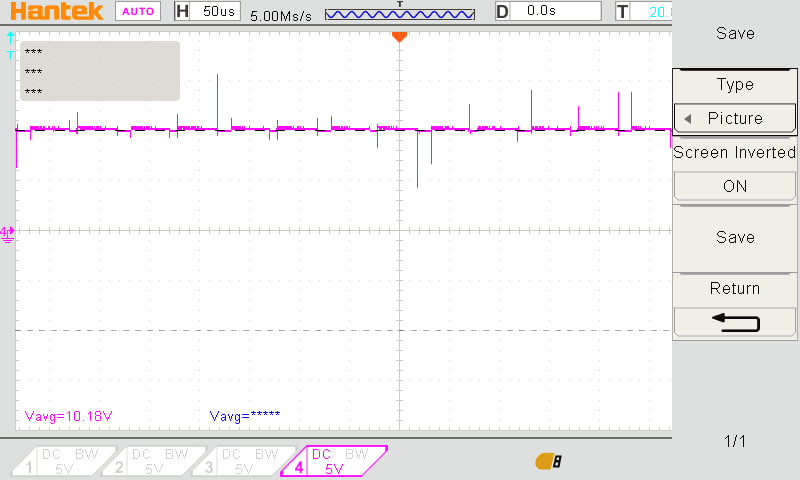
\includegraphics[width=\linewidth]{Figures/02.jpg} % Place photo for second duty/load condition here
        \caption{$V_{out}$ at 0.6 duty.}
        \label{fig:hysteresis_v_d2}
    \end{subfigure}
    \label{fig:hysteresis_voltage_results}
    \centering
    \begin{subfigure}[b]{0.45\textwidth}
        \centering
        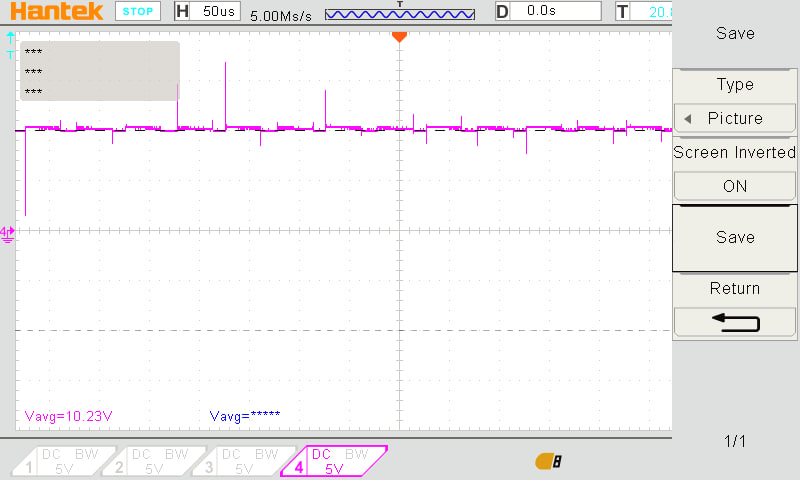
\includegraphics[width=\linewidth]{Figures/03.jpg} % Place photo for first duty/load condition here
        \caption{$V_{out}$ at 0.65 duty.}
        \label{fig:hysteresis_v_d1}
    \end{subfigure}
    \hfill
    \begin{subfigure}[b]{0.45\textwidth}
        \centering
        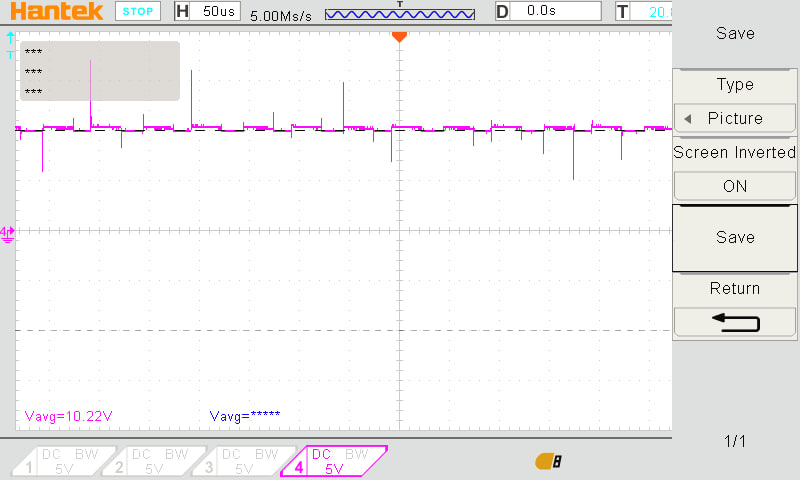
\includegraphics[width=\linewidth]{Figures/04.jpg} % Place photo for second duty/load condition here
        \caption{$V_{out}$ at 0.7 duty.}
        \label{fig:hysteresis_v_d2}
    \end{subfigure}
    \label{fig:hysteresis_voltage_results}
    \centering
    \begin{subfigure}[b]{0.45\textwidth}
        \centering
        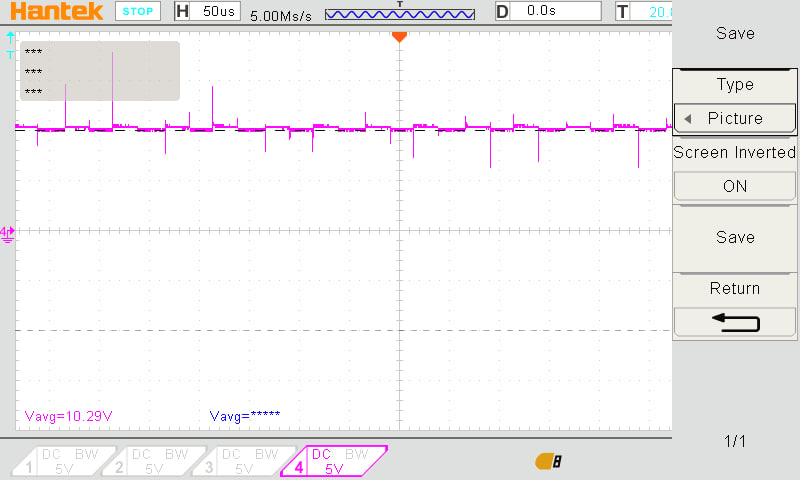
\includegraphics[width=\linewidth]{Figures/05.jpg} % Place photo for first duty/load condition here
        \caption{$V_{out}$ at 0.75 duty.}
        \label{fig:hysteresis_v_d1}
    \end{subfigure}
    \hfill
    \begin{subfigure}[b]{0.45\textwidth}
        \centering
        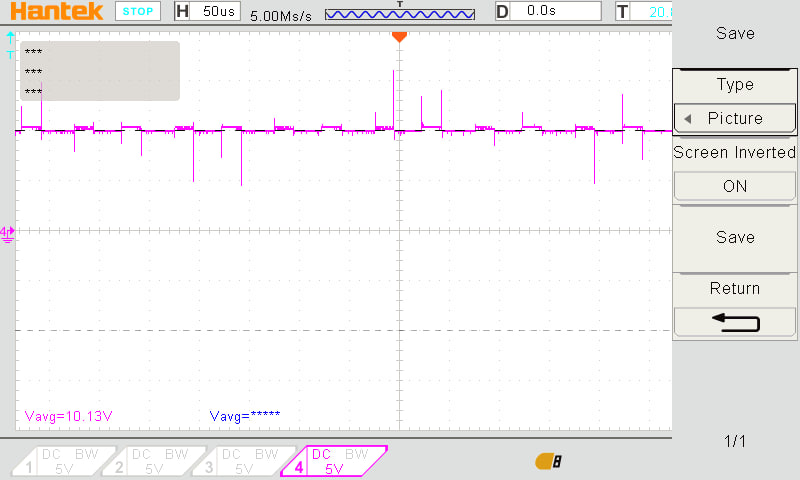
\includegraphics[width=\linewidth]{Figures/06.jpg} % Place photo for second duty/load condition here
        \caption{$V_{out}$ at 0.8 duty.}
        \label{fig:hysteresis_v_d2}
    \end{subfigure}
    \label{fig:hysteresis_voltage_results}
    \centering
    \begin{subfigure}[b]{0.45\textwidth}
        \centering
        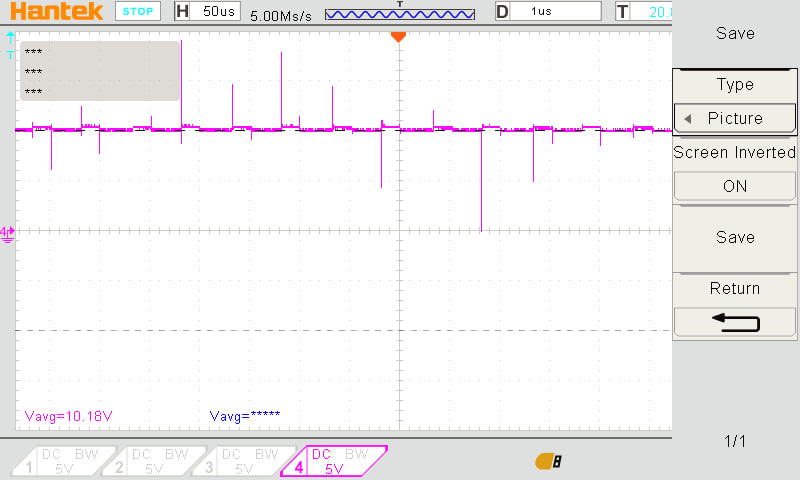
\includegraphics[width=\linewidth]{Figures/07.jpg} % Place photo for first duty/load condition here
        \caption{$V_{out}$ at 0.82 duty.}
        \label{fig:hysteresis_v_d1}
    \end{subfigure}
    \hfill
    \begin{subfigure}[b]{0.45\textwidth}
        \centering
        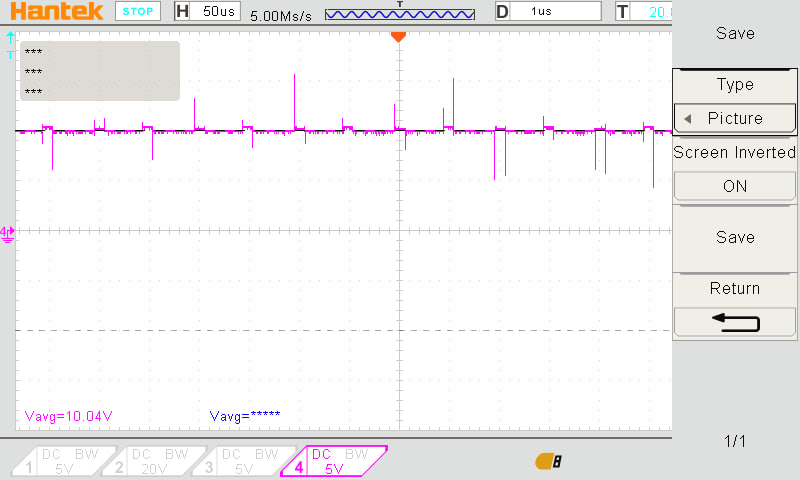
\includegraphics[width=\linewidth]{Figures/08.jpg} % Place photo for second duty/load condition here
        \caption{$V_{out}$ at 0.9 duty.}
        \label{fig:hysteresis_v_d2}
    \end{subfigure}
    \caption{$V_{out}$ at different duties.}
    \label{fig:hysteresis_voltage_results}
\end{figure}
The experimental hardware waveforms captured during these step-load transitions are displayed in Figure \ref{fig:hysteresis_voltage_results}. The results confirm that when the switch toggles the series $47\ \Omega$ branch active, the control loop tracks the transient profile. It automatically adjusts the operating limits within milliseconds, keeping the voltage ripple bounded within its configured tolerance envelope and maintaining a stable 10\text{ V} bus line.

\subsection{Maximum Power Point Tracking (MPPT) Control}
While clamping the intermediate bus voltage via hysteresis logic ensures load-side stabilization, optimizing the source generation side requires overriding static operation to counteract dynamic environmental shifts. To extract the maximum possible energy from the non-linear photovoltaic characteristic curve, the converter's control core must adapt dynamically to atmospheric fluctuations and solar irradiance levels.

This supervisory control layer integrates an automated Perturb and Observe (P\&O) Maximum Power Point Tracking (MPPT) algorithm. The microcontroller continuously samples both the instantaneous panel output voltage ($V_{pv}$) and panel output current ($I_{pv}$) via the sensing infrastructure. The control routine evaluates the digital tracking parameters to calculate the instantaneous power derivative ($dP/dV$). If this derivative is non-zero, the system recognizes that the current operating point deviates from the peak electrochemical power ceiling.

\subsubsection{}section{Discrete Open-Loop Characterization (Manual Duty Cycle Cases)}
To map the physical operating trajectory along the non-linear PV characteristic curve before engaging the automated engine, steady-state experimental testing was conducted across eight discrete manual duty cycle steps. Modulating these boundary constraints shifts the apparent input impedance of the Interleaved Boost Converter, forcing the panel operating point ($V_{pv}$, $I_{pv}$) to adapt dynamically. The empirical results for each operating case are detailed below:

\paragraph{Case 1: Duty Cycle $D = 0.50$}

\begin{figure}[H]
    \centering
    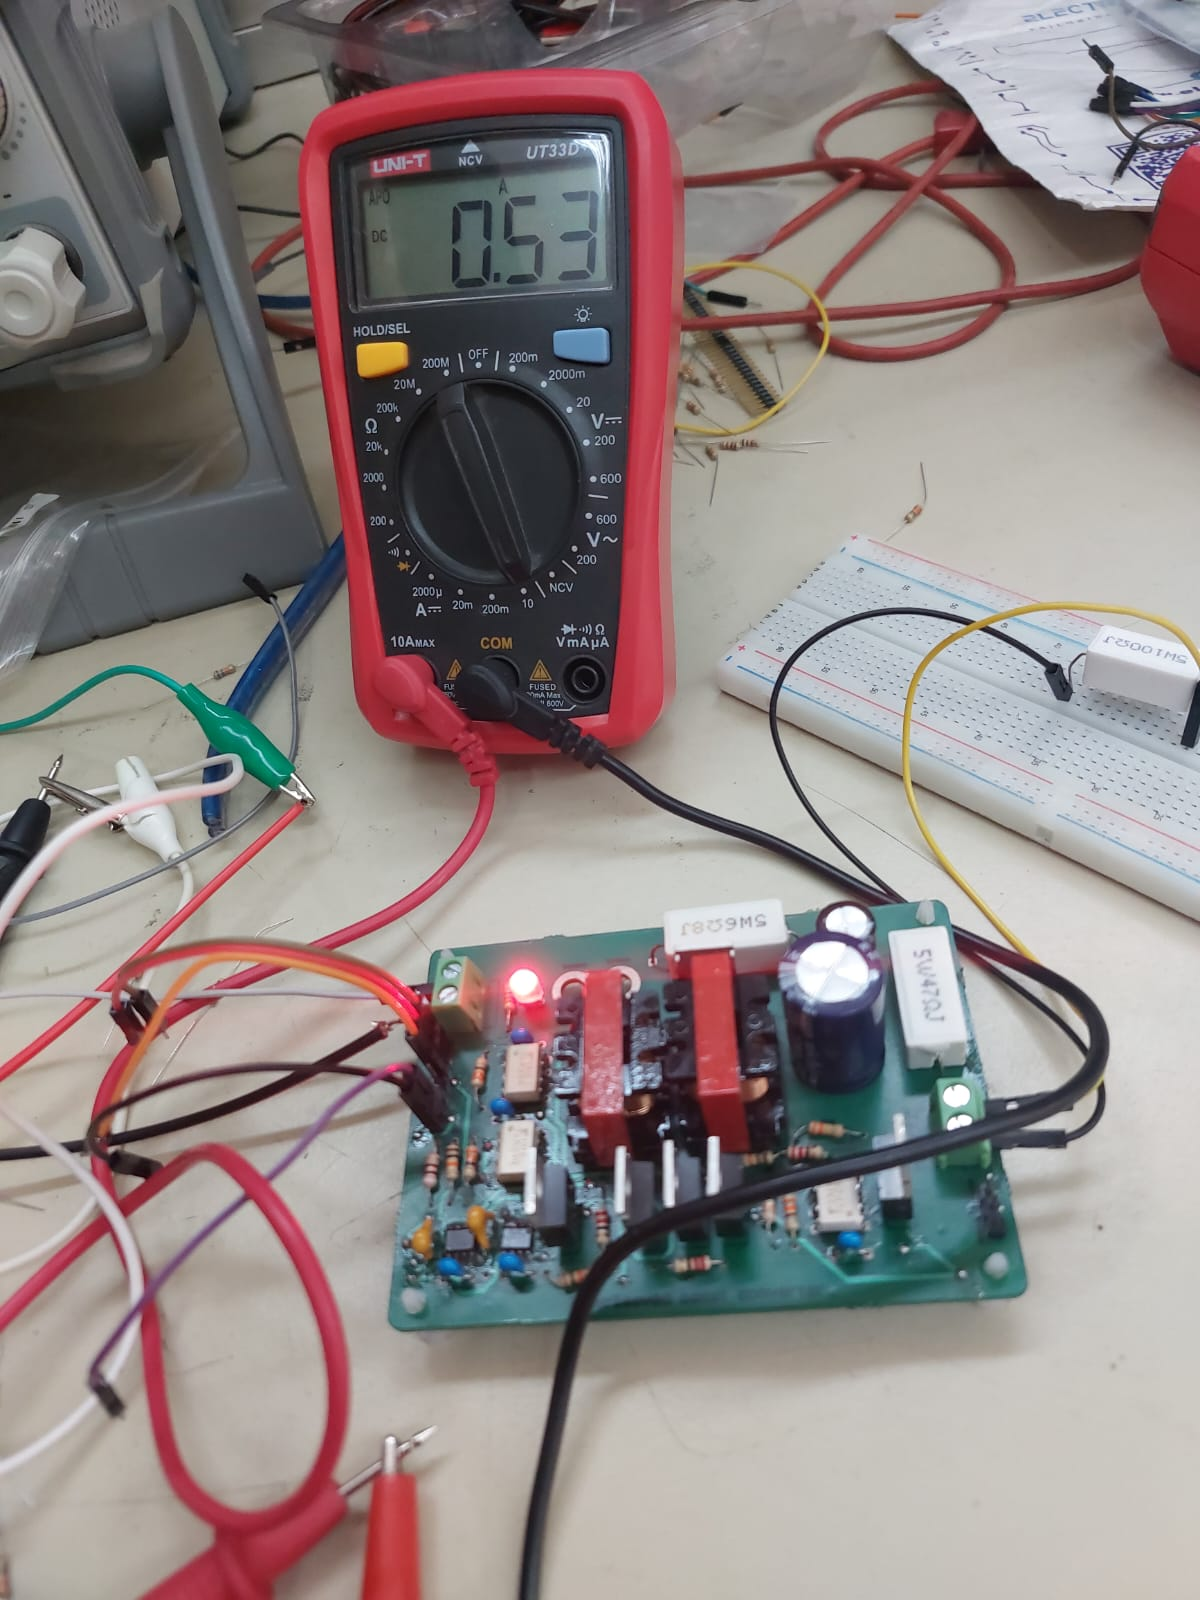
\includegraphics[width=0.4\textwidth]{Figures/pv1.jpeg}
    \caption{Experimental hardware tracking waveforms of $V_{pv}$ and $I_{pv}$ at a static duty cycle $D = 0.50$.}
    \label{fig:pv_case_d050}
\end{figure}
Under this operating state, the input parameters settle to their respective open-loop equilibrium points. The total input power extracted from the PV source is quantified via the electrical power equation:
\begin{equation}
    P_{pv1} = 0.53 \times 7.8 = 4.13W
\end{equation}
\paragraph{Case 2: Duty Cycle $D = 0.60$}
Increasing the conduction interval shifts the converter's transformation ratio, modifying the current drawn from the cells. The matching input power conversion is given by:
\begin{equation}
    P_{pv2} = 0.64 \times 7.048 = 4.51W
\end{equation}

\begin{figure}[H]
    \centering
    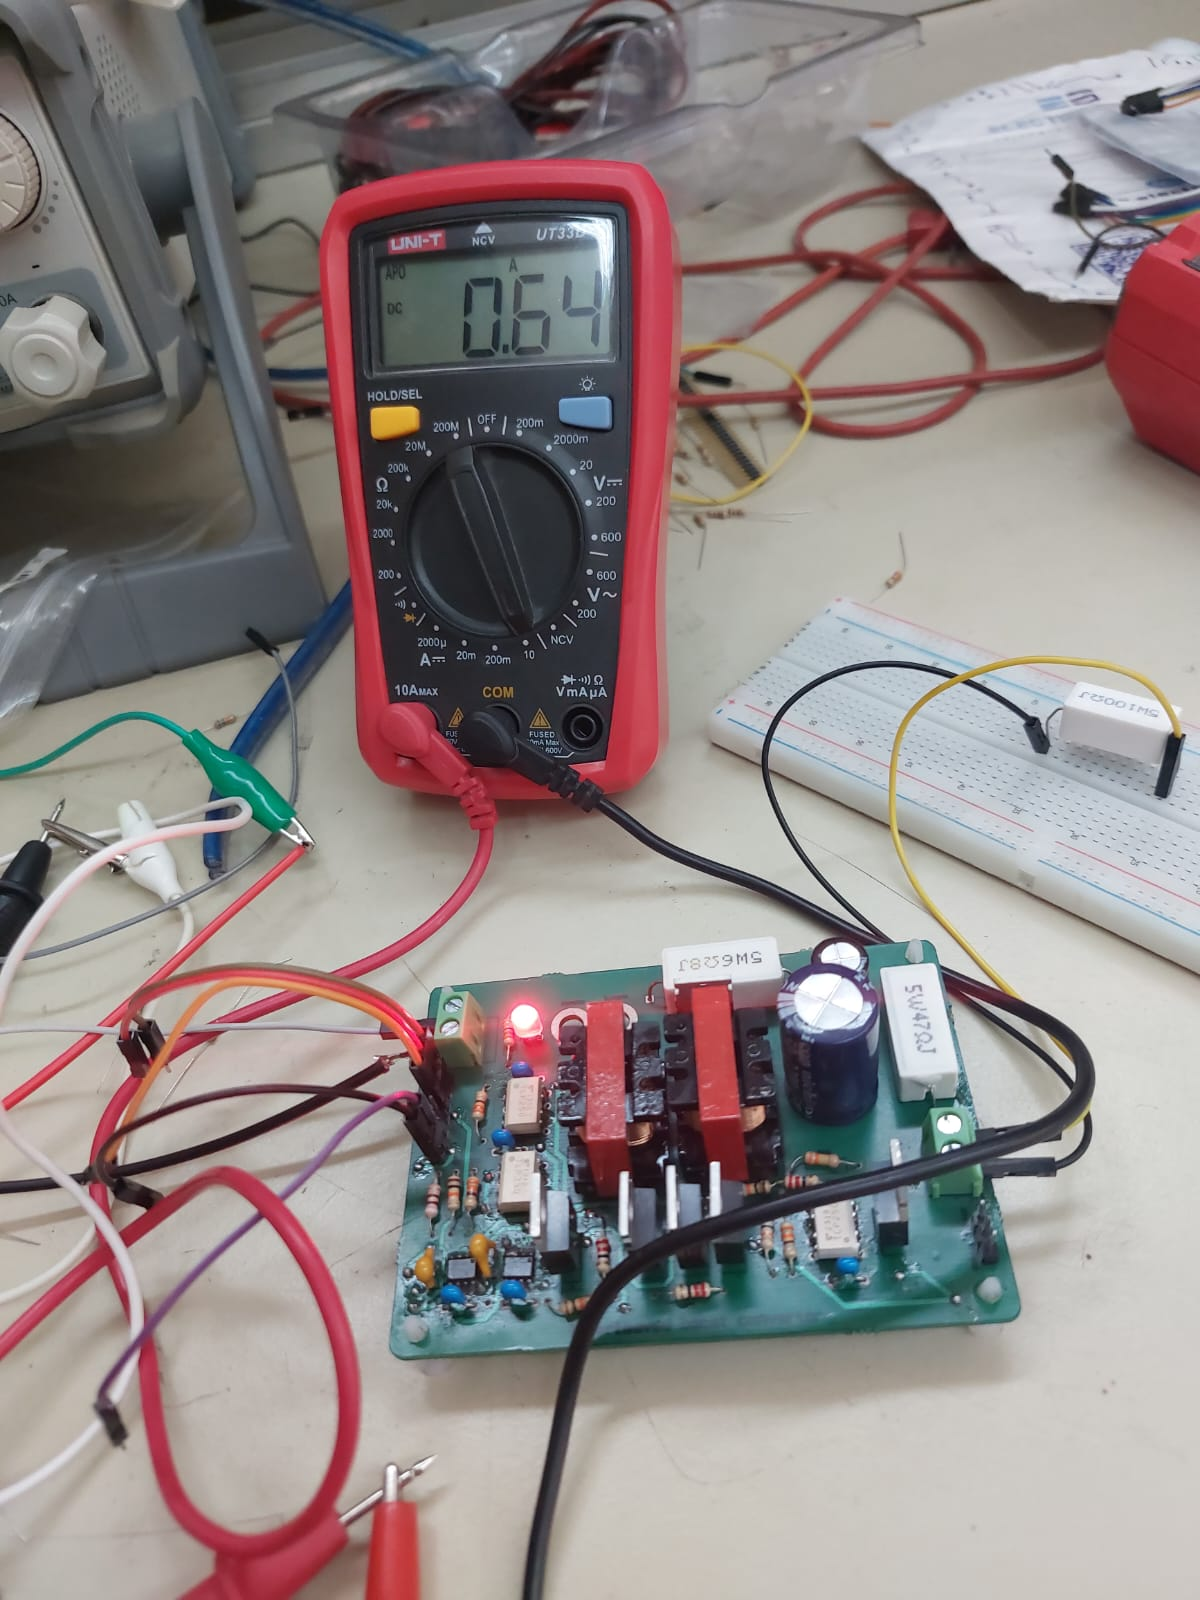
\includegraphics[width=0.7\textwidth]{Figures/pv2.jpeg}
    \caption{Experimental hardware tracking waveforms of $V_{pv}$ and $I_{pv}$ at a static duty cycle $D = 0.60$.}
    \label{fig:pv_case_d060}
\end{figure}
\newpage
\paragraph{Case 3: Duty Cycle $D = 0.65$}
Fine adjustments to the switching periods shift the electrical profile closer toward the knee of the panel's characteristic curve. The steady-state power relation is evaluated as:
\begin{equation}
    P_{pv3} = 0.68 \times 6.776 = 4.608W
\end{equation}

\begin{figure}[H]
    \centering
    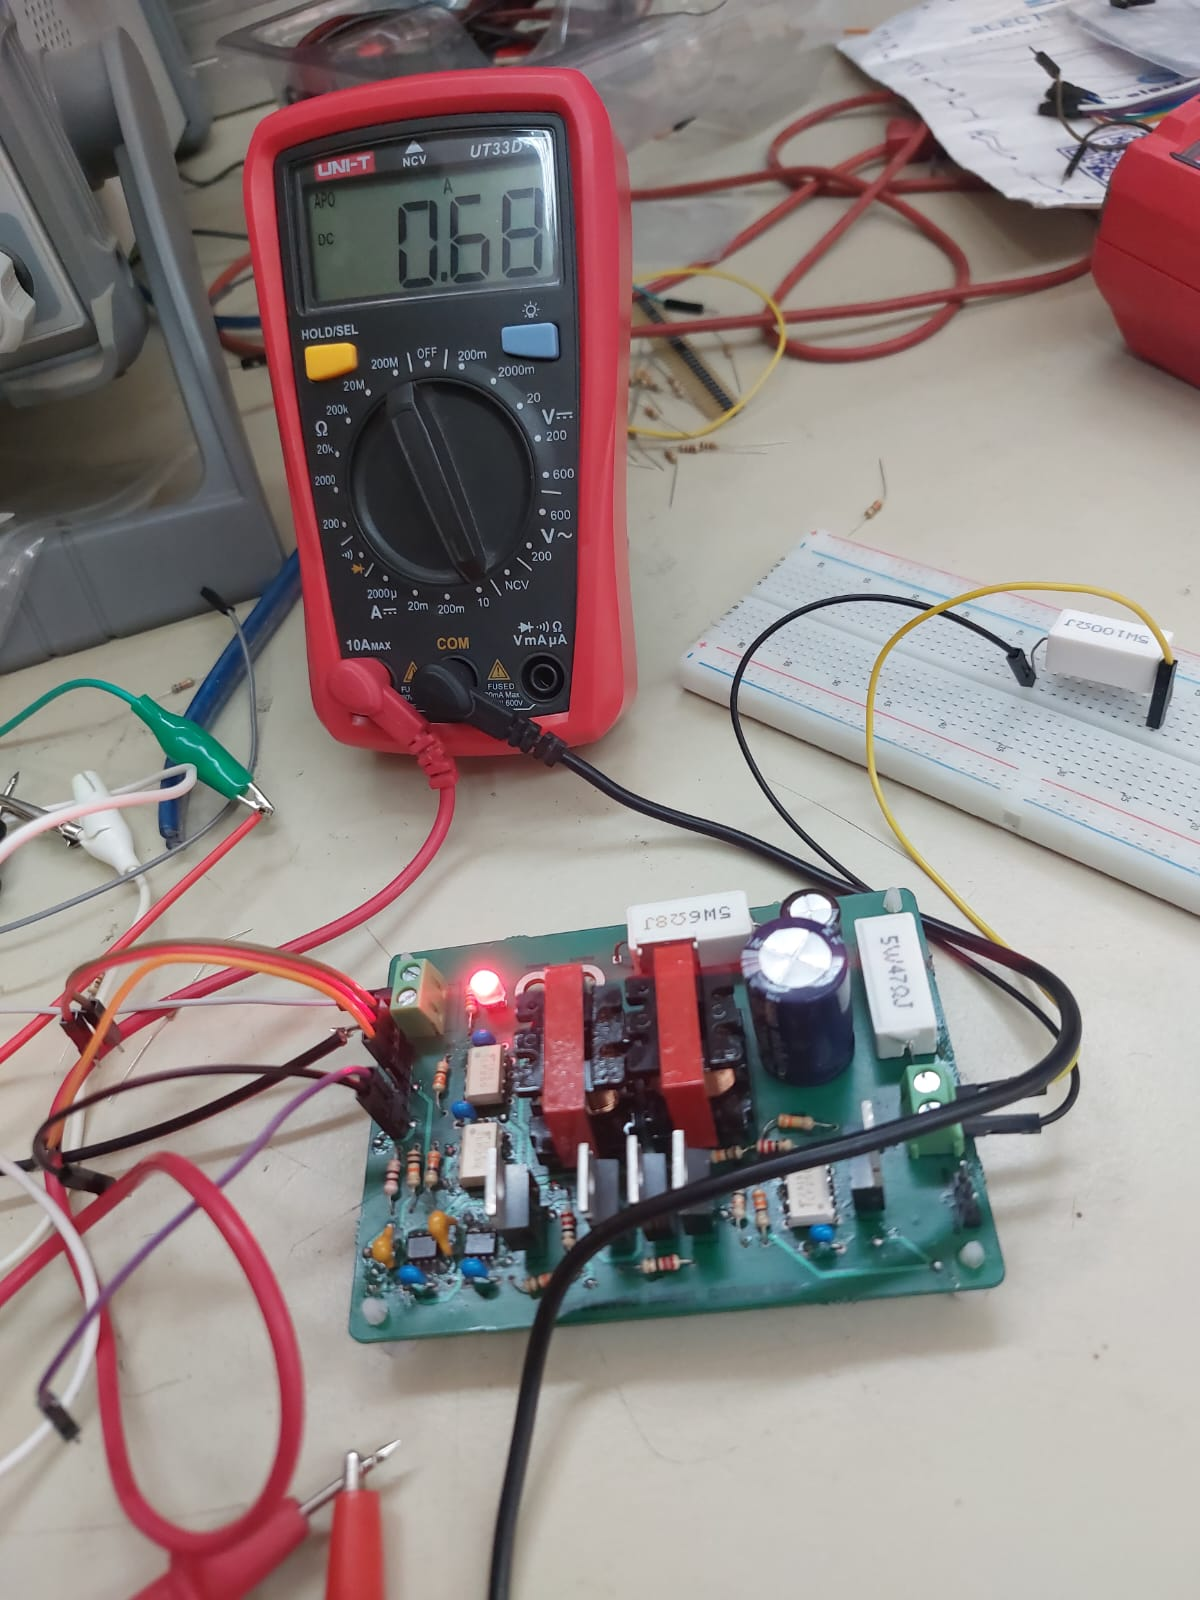
\includegraphics[width=0.7\textwidth]{Figures/pv3.jpeg}
    \caption{Experimental hardware tracking waveforms of $V_{pv}$ and $I_{pv}$ at a static duty cycle $D = 0.65$.}
    \label{fig:pv_case_d065}
\end{figure}
\newpage
\paragraph{Case 4: Duty Cycle $D = 0.70$}
At this boundary index, the operational vector approaches the nominal design parameters of the array interface. The calculated electrical power delivery is expressed by:
\begin{equation}
    P_{pv4} = {0.74 \times 6.368 = 4.712W}
\end{equation}

\begin{figure}[H]
    \centering
    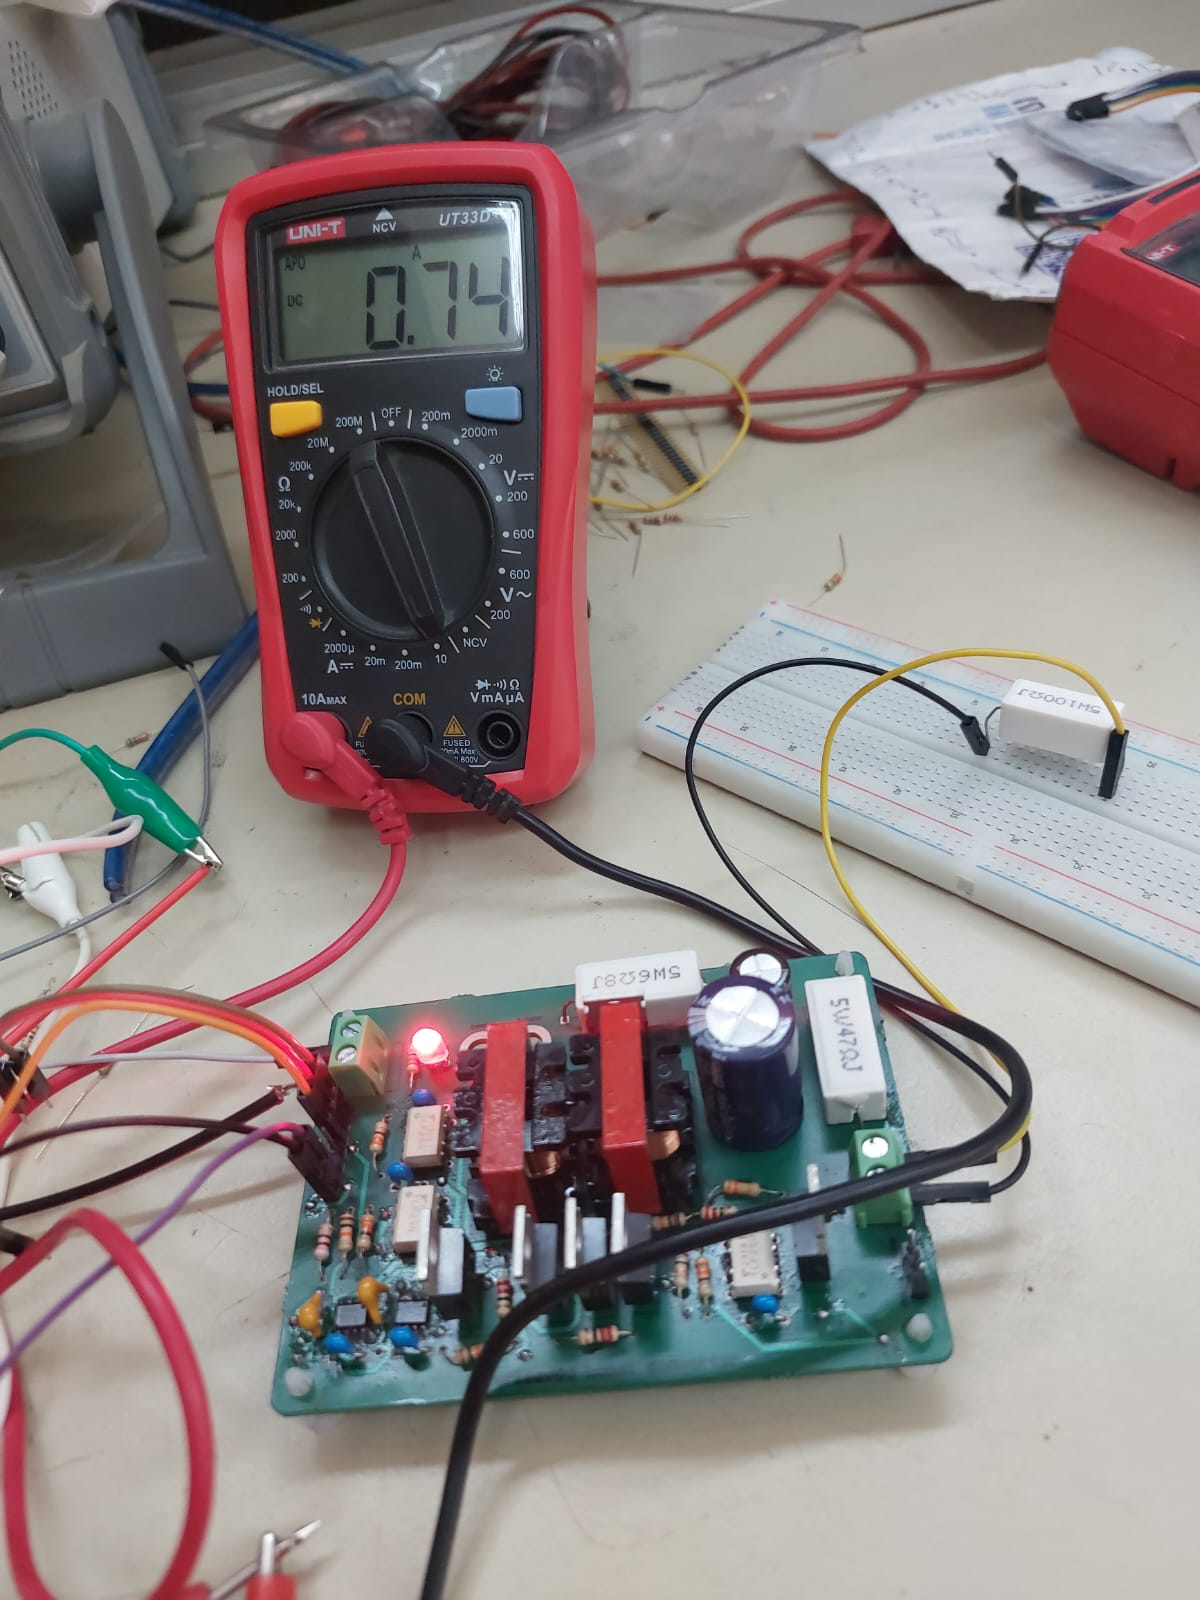
\includegraphics[width=0.7\textwidth]{Figures/pv4.jpeg}
    \caption{Experimental hardware tracking waveforms of $V_{pv}$ and $I_{pv}$ at a static duty cycle $D = 0.70$.}
    \label{fig:pv_case_d070}
\end{figure}
\newpage
\paragraph{Case 5: Duty Cycle $D = 0.75$}
Further incrementation alters the impedance matching condition, driving changes across the terminal metrics. The electrical source performance yields:
\begin{equation}
    P_{pv5} = 0.79 \times 6.096 = 4.75488W
\end{equation}

\begin{figure}[H]
    \centering
    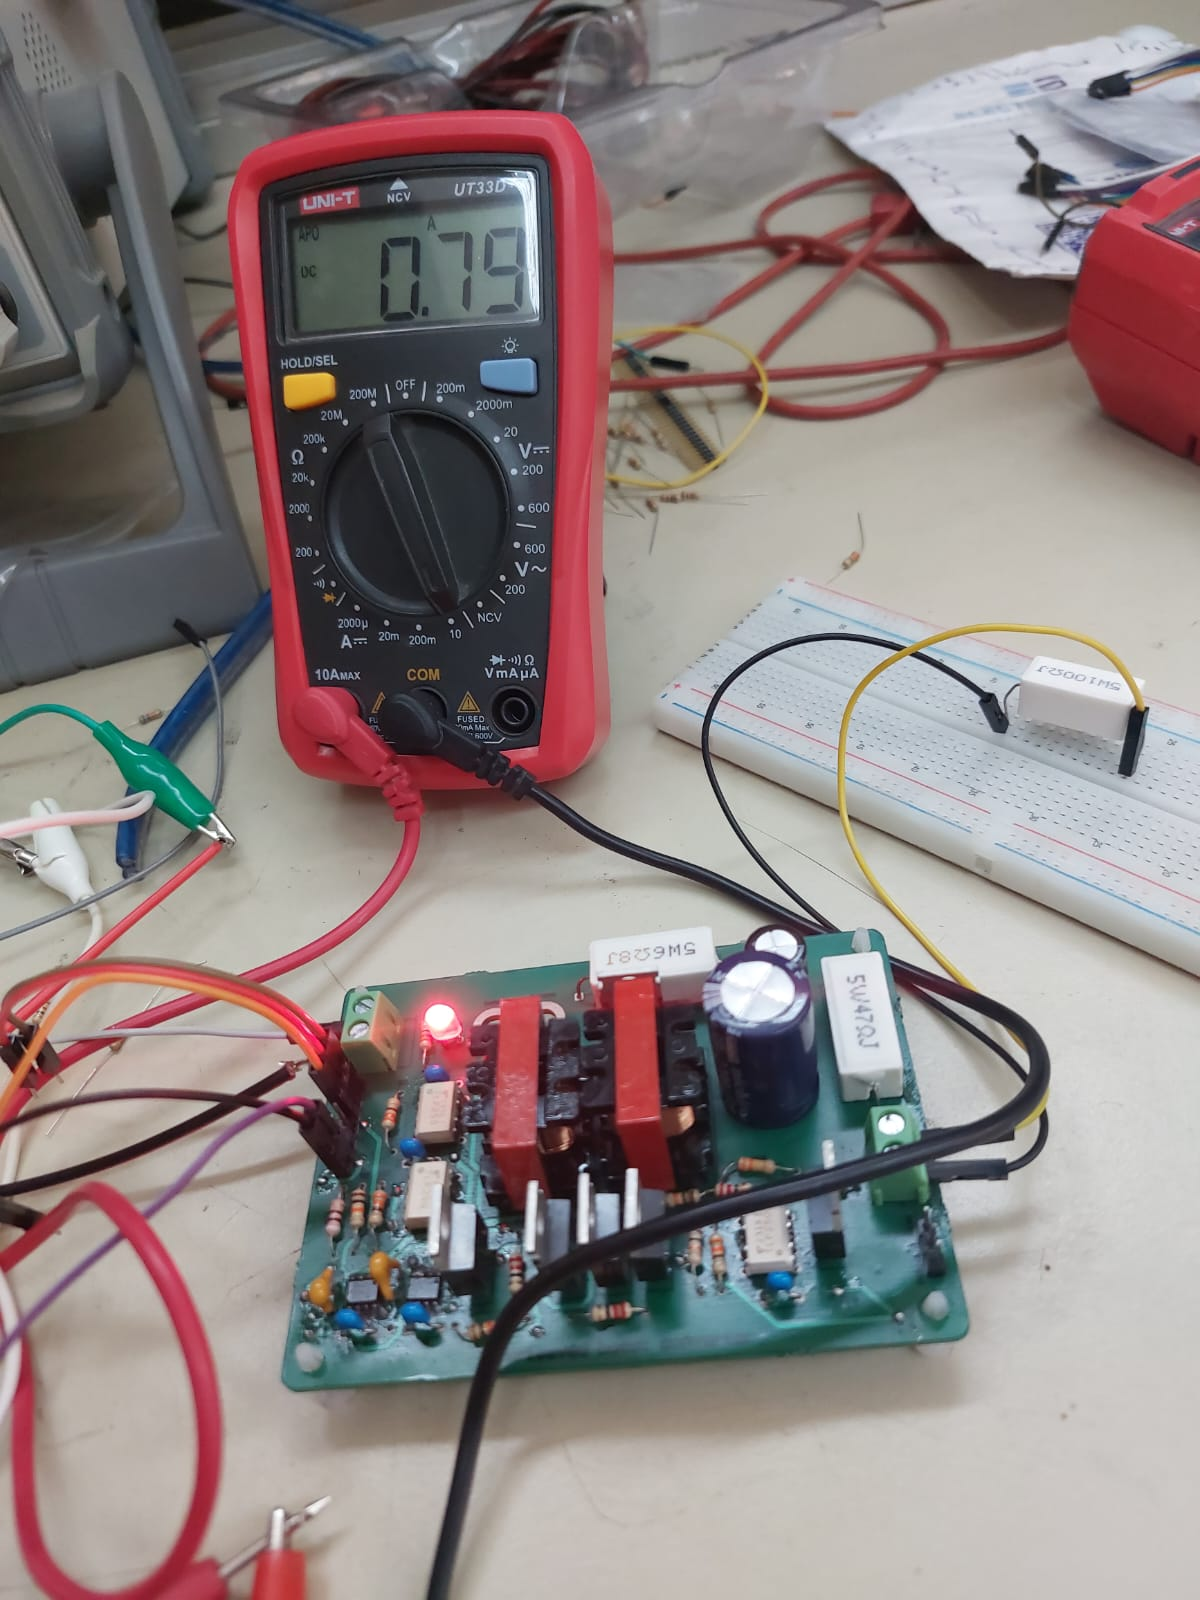
\includegraphics[width=0.7\textwidth]{Figures/pv5.jpeg}
    \caption{Experimental hardware tracking waveforms of $V_{pv}$ and $I_{pv}$ at a static duty cycle $D = 0.75$.}
    \label{fig:pv_case_d075}
\end{figure}
\newpage
\paragraph{Case 6: Duty Cycle $D = 0.77$}
Operating at higher conversion bounds significantly restricts the cell voltage profile while maximizing current displacement. The input power calculation is defined by:
\begin{equation}
    P_{pv6} = 0.81 \times 5.892 = 4.772W
\end{equation}

\begin{figure}[H]
    \centering
    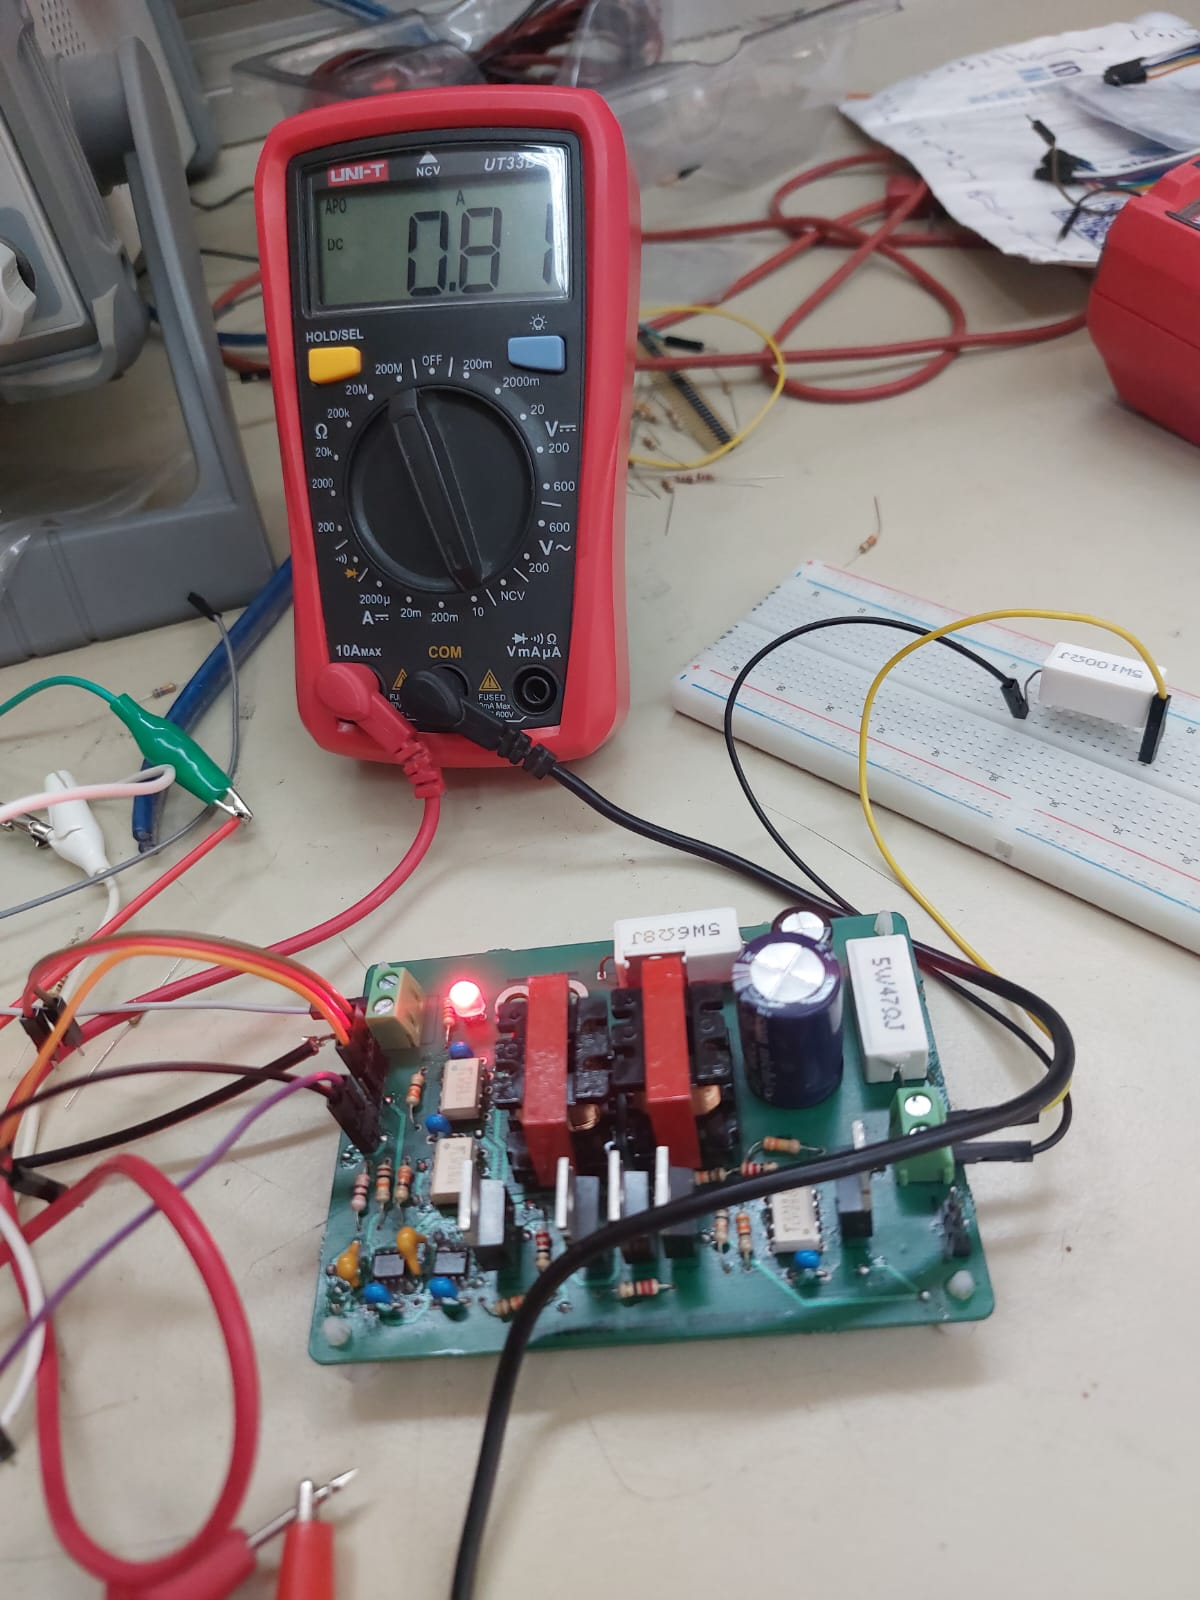
\includegraphics[width=0.7\textwidth]{Figures/pv6.jpeg}
    \caption{Experimental hardware tracking waveforms of $V_{pv}$ and $I_{pv}$ at a static duty cycle $D = 0.77$.}
    \label{fig:pv_case_d080}
\end{figure}
\newpage
\paragraph{Case 7: Duty Cycle $D = 0.8$}
This operational state benchmarks the system tracking bounds right before extreme voltage degradation thresholds are crossed. The localized equation yields:
\begin{equation}
    P_{pv7} = 0.84 \times 5.688 = 4.777W
\end{equation}

\begin{figure}[H]
    \centering
    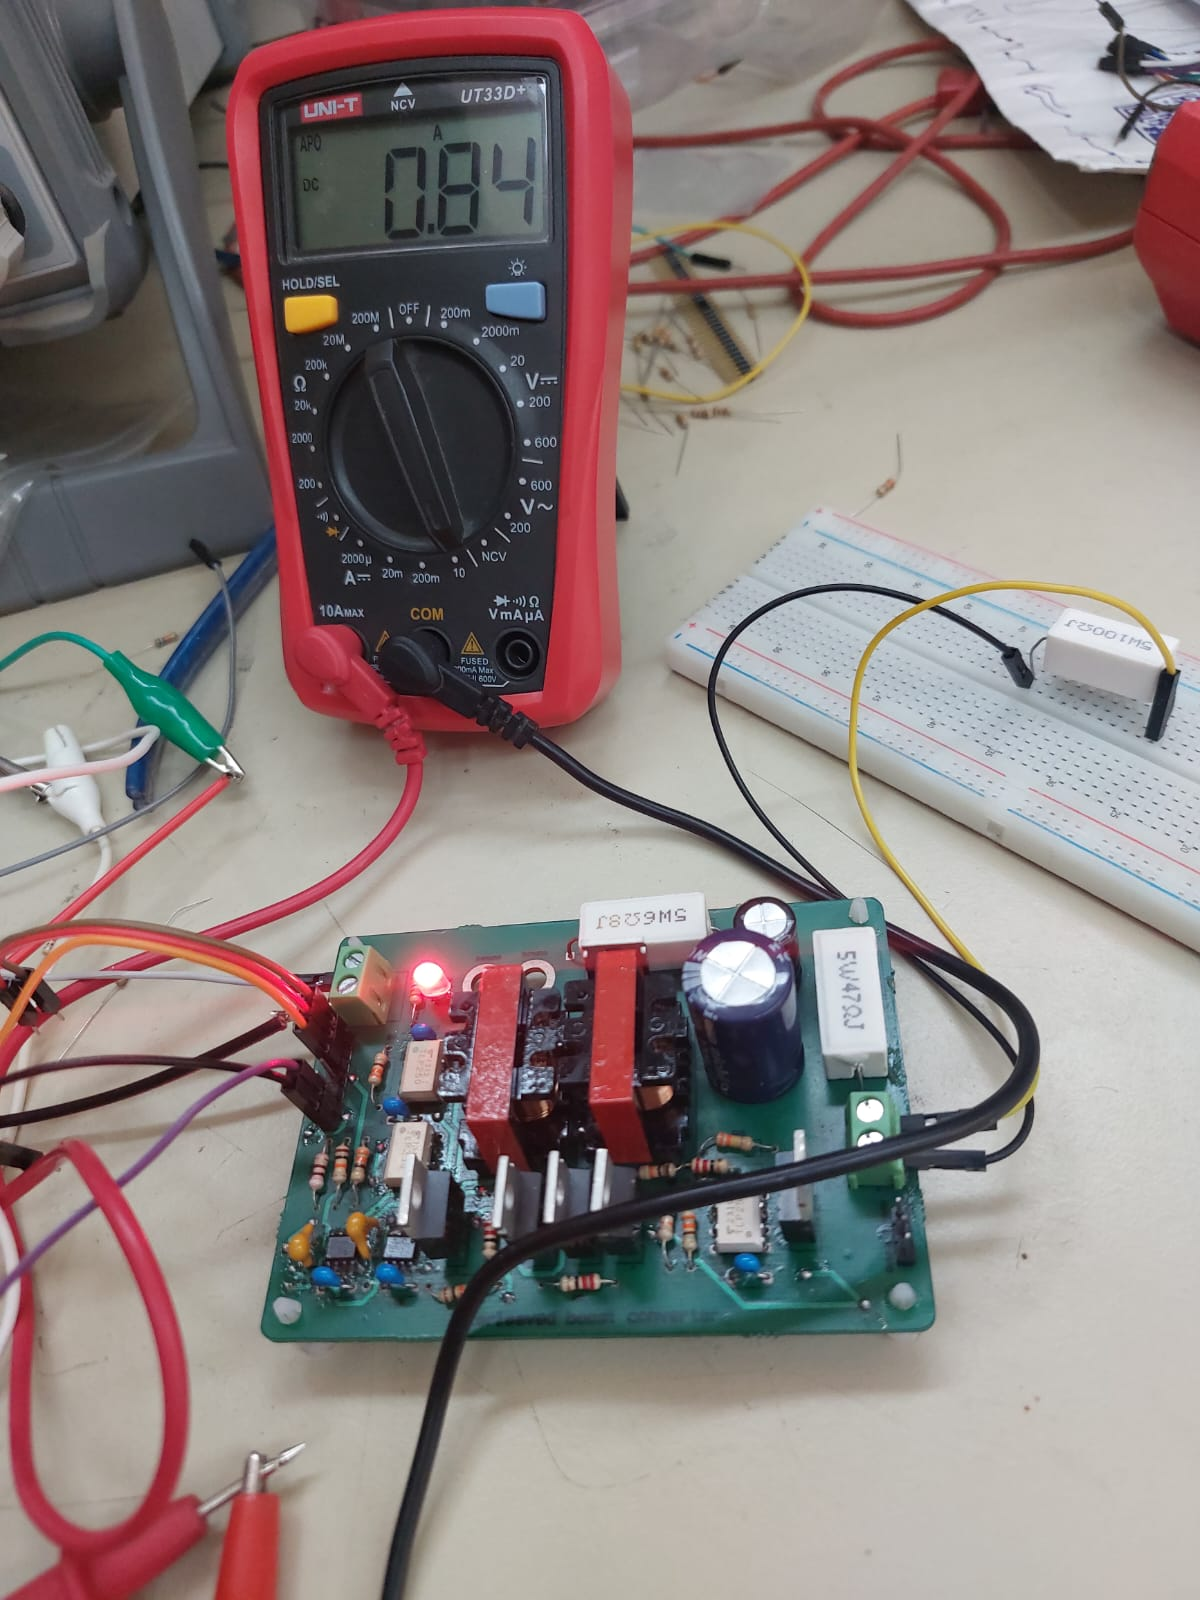
\includegraphics[width=0.7\textwidth]{Figures/pv7.jpeg}
    \caption{Experimental hardware tracking waveforms of $V_{pv}$ and $I_{pv}$ at a static duty cycle $D = 0.8$.}
    \label{fig:pv_case_d082}
\end{figure}
\newpage
\paragraph{Case 8: Duty Cycle $D = 0.85$}
At this extreme conduction threshold, the panel operates deeply within its voltage-collapse region, revealing low generation yields due to poor impedance alignment. The ultimate manual tracking step is quantified as:
\begin{equation}
    P_{pv8} = 0.88 \times 5.416 = 4.766W
\end{equation}

\begin{figure}[H]
    \centering
    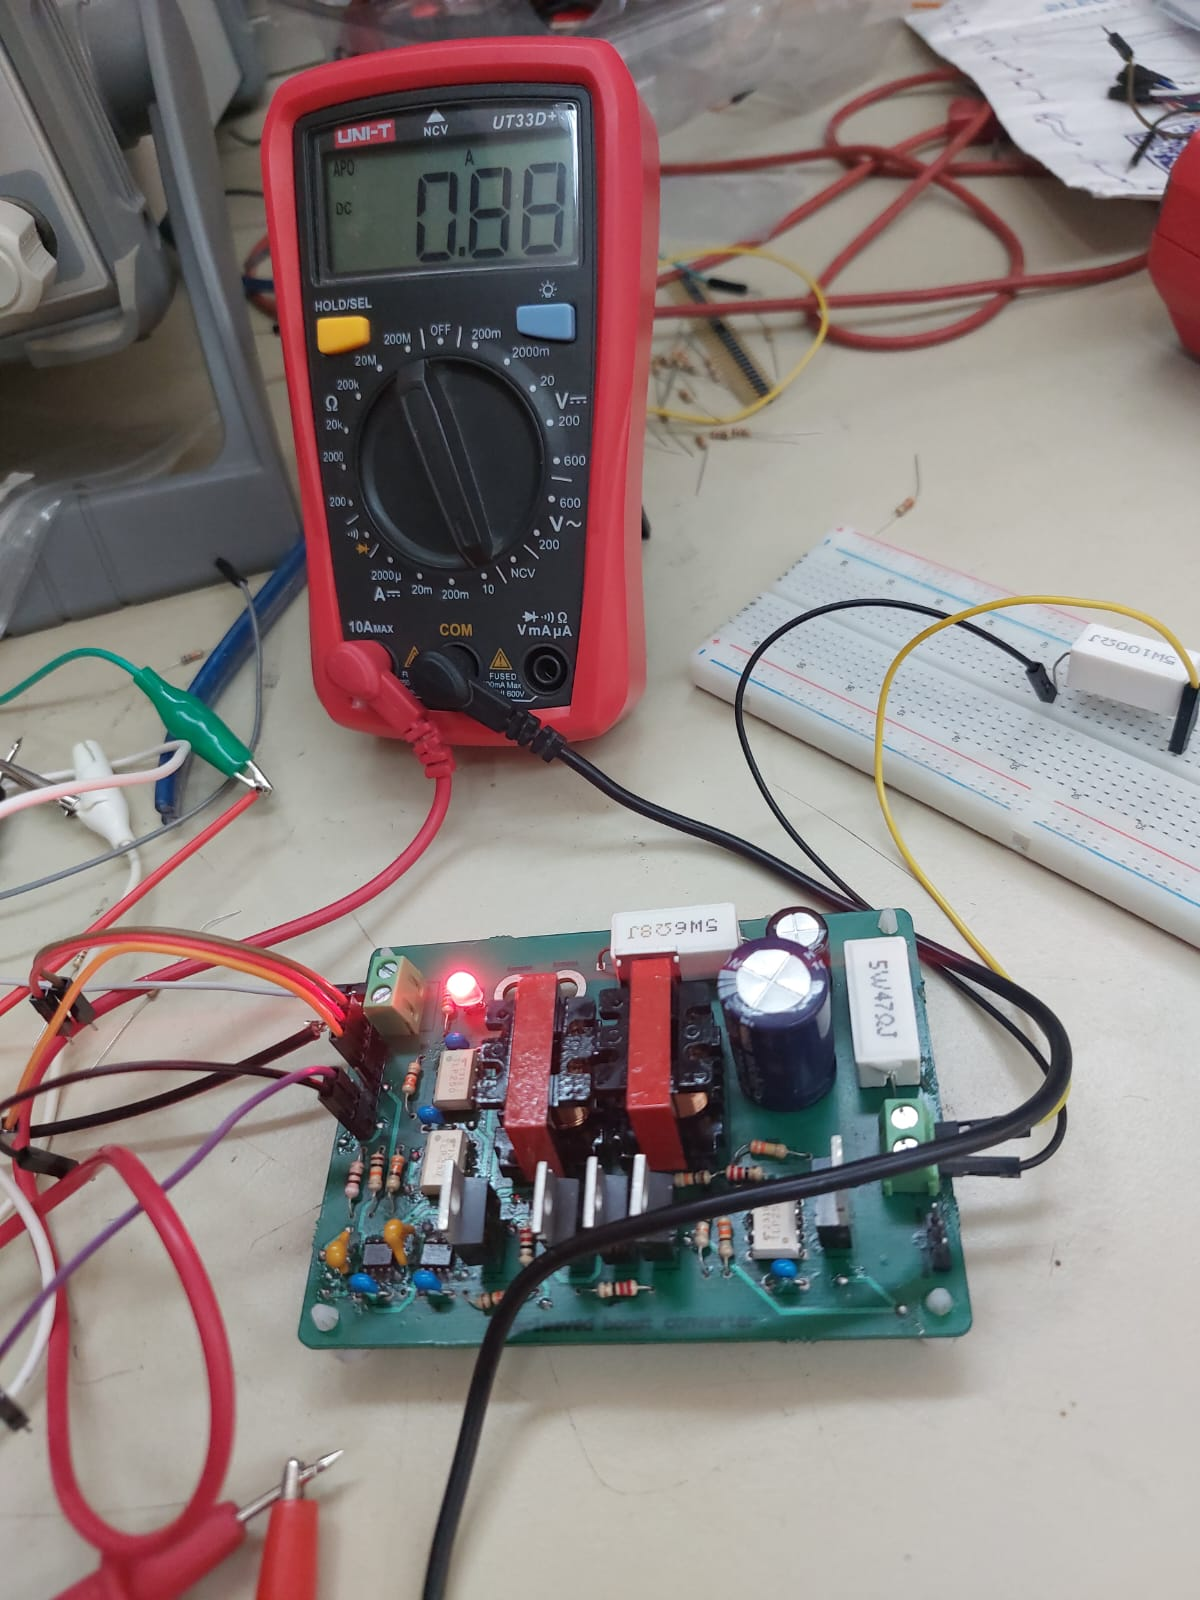
\includegraphics[width=0.7\textwidth]{Figures/pv8.jpeg}
    \caption{Experimental hardware tracking waveforms of $V_{pv}$ and $I_{pv}$ at an extreme static duty cycle $D = 0.85$.}
    \label{fig:pv_case_d090}
\end{figure}

Based on manual calculation, we can estimate that the maximum power occurs at around duty 0.77 to 0.8.
An automatic MPPT Control is utilized to find this maximum point automatically.
\newpage
\subsection{Automated Embedded MPPT Optimization Engine}
Manual manipulation of the duty cycle verifies that static switching parameters cannot accommodate real-time environmental variations. To resolve this limitation, the hardware system transitions from discrete configuration to an autonomous, dual-stage embedded tracking engine executed by the central microcontroller infrastructure.

The embedded control implementation relies on a hybrid algorithmic approach divided into two distinct operational execution layers:
\begin{enumerate}
    \item \textbf{Global Sweep Optimization Tracking Phase:} Upon initialization, the converter executes an automated sweeping routine across a safe duty cycle range ($D = 0.20$ to $D = 0.90$). By systematically incrementing the PWM register targets via fixed steps, the system logs the absolute electrical power profile to locate and record the Global Maximum Power Point (GMPP), completely bypassing any localized sub-peaks caused by transient dynamics.
    \item \textbf{Perturb and Observe (P\&O) Fine-Tracking Adaptive Phase:} Once the sweep terminates, the engine locks onto the recorded peak duty cycle ticks as its nominal baseline. It then seamlessly activates a continuous P\&O loop. The routine samples high-frequency ADC current and voltage variables, calculates the dynamic power differential ($\Delta P$), and adaptively perturbs the hardware duty targets via micro-adjustments ($\pm \Delta D$) to lock the hardware directly at the peak efficiency vertex ($dP/dV = 0$).
\end{enumerate}

To guarantee hardware accuracy, the interleaved 180$^\circ$ phase-shifted pulse train is configured via low-level hardware register access utilizing Phase and Frequency Correct PWM mode under Timer 1. Inter-phase switching synchronization is handled dynamically via an embedded Interrupt Service Routine (ISR) triggered via the \texttt{TIMER1\_COMPB\_vect} vector mask.

The complete physical firmware architecture deployed to execute the automatic tracking sequence is detailed in the algorithmic code implementation module below:

\begin{lstlisting}[language=C++, caption={Embedded Arduino C++ Hybrid Global Sweep and P\&O MPPT Firmware Architecture.}, label={lst:mppt_arduino_firmware}]
// Embedded MPPT Core Control Firmware -- Interleaved Boost Converter Layout
const int voltagePin = A0;
const int currentPin = A1;

// Sensor calibration constants
const float V_CONVERSION = 0.0654;
const float ACS_OFFSET   = 514.3;
const float ACS_SENS     = 0.2121;

// Hardware Timer register parameters
const unsigned int TOTAL_TICKS = 1600; // Defines PWM period base frequency
unsigned int currentDutyTicks = 320; 
unsigned int bestDutyTicks = 320;
float maxPowerFound = 0.0;
bool isSweeping = true;

unsigned long prevMillis = 0;
const int sweepStep = 16; 
const int sweepDelay = 150; 

float prevPower = 0.0;
int perturbDirection = 1;
const int perturbStep = 4; // Step resolution for closed-loop fine tracking

void setup() {
  pinMode(9, OUTPUT);  % Phase 1 Gate Output
  pinMode(10, OUTPUT); % Phase 2 Gate Output

  % Reset Timer 1 Control Registers
  TCCR1A = 0;
  TCCR1B = 0;
  TCNT1  = 0;

  % Configure Phase and Frequency Correct PWM Mode (Mode 9)
  TCCR1A |= (1 << WGM11);
  TCCR1B |= (1 << WGM13) | (1 << WGM12);

  % Enable non-inverting PWM output on Channel A (Pin 9)
  TCCR1A |= (1 << COM1A1);
  TCCR1A &= ~((1 << COM1B1) | (1 << COM1B0));

  % Set top boundary and initial duty cycle tracking variables
  ICR1 = TOTAL_TICKS;
  OCR1A = currentDutyTicks;
  OCR1B = TOTAL_TICKS / 2; % Symmetrical trigger for phase interleave ISR

  % Activate Timer 1 Compare Match B interrupt
  TIMSK1 |= (1 << OCIE1B);
  TCCR1B |= (1 << CS10); % No prescaling for optimal high-frequency switching

  Serial.begin(115200);
  Serial.println("=================================================");
  Serial.println("   MPPT Interleaved Boost -- Starting Sweep");
  Serial.println("=================================================");
  Serial.println("Duty\tTicks\tV_pv(V)\t\tI_pv(A)\t\tP_pv(W)");
}

% Interrupt Service Routine for interleaved 180-degree phase shift execution
ISR(TIMER1_COMPB_vect) {
  PORTB |= (1 << PORTB2); % Fire high-frequency trigger flag
  
  unsigned int currentDuty = OCR1A;
  
  % Hardware tracking loop synchronization loop
  while (TCNT1 < (TOTAL_TICKS / 2) + currentDuty) {
    if (TCNT1 < (TOTAL_TICKS / 2) && TCNT1 >= (currentDuty - (TOTAL_TICKS / 2))) {
      break;
    }
  }

  PORTB &= ~(1 << PORTB2); % Clear trigger flag
}

% Oversampled digital filter function for analog signal noise attenuation
float readAveragedADC(int pin, int samples = 64) {
  long sum = 0;
  for (int i = 0; i < samples; i++) {
    sum += analogRead(pin);
    delayMicroseconds(50);
  }
  return sum / (float)samples;
}

void loop() {
  if (isSweeping) {
    % --- STAGE 1: GLOBAL SWEEP TRACE OVER THE PV BOUNDARIES ---
    if (millis() - prevMillis >= sweepDelay) {
      prevMillis = millis();

      float pvVoltage = readAveragedADC(voltagePin) * V_CONVERSION;
      float rawCurrent = readAveragedADC(currentPin);
      float Iactual = (rawCurrent - ACS_OFFSET) * (5.0 / 1023.0) / ACS_SENS;
      if (Iactual < 0) Iactual = 0;
      
      float pvPower = pvVoltage * Iactual;
      float activeDuty = (float)currentDutyTicks / TOTAL_TICKS;

      Serial.print(activeDuty, 2);   Serial.print("\t");
      Serial.print(currentDutyTicks); Serial.print("\t");
      Serial.print(pvVoltage, 2);     Serial.print("\t\t");
      Serial.print(Iactual, 3);       Serial.print("\t\t");
      Serial.println(pvPower, 2);

      % Record maximum power envelope
      if (pvPower > maxPowerFound) {
        maxPowerFound = pvPower;
        bestDutyTicks = currentDutyTicks;
      }

      currentDutyTicks += sweepStep;
      
      % Evaluate sweep completion status
      if (currentDutyTicks > 1440) { 
        isSweeping = false;
        currentDutyTicks = bestDutyTicks;
        OCR1A = currentDutyTicks; % Lock hardware to peak point duty
        prevPower = maxPowerFound;
        
        Serial.println("-------------------------------------------------");
        Serial.print("SWEEP DONE! Peak Power : "); 
        Serial.print(maxPowerFound, 2);
        Serial.println(" W");
        Serial.print("Locking at ticks       : "); Serial.print(bestDutyTicks);
        Serial.print(((float)bestDutyTicks / TOTAL_TICKS) * 100.0, 1); 
        Serial.println("% Duty)");
        Serial.println("-------------------------------------------------");
        Serial.println("Entering P&O fine-tracking...");
        Serial.println("Dir\tTicks\tV_pv(V)\t\tI_pv(A)\t\tP_pv(W)");
      } else {
        OCR1A = currentDutyTicks;
      }
    }
  } else {
    % --- STAGE 2: CLOSED-LOOP PERTURB & OBSERVE FINE REGULATION ---
    if (millis() - prevMillis >= 1500) {
      prevMillis = millis();

      float pvVoltage = readAveragedADC(voltagePin) * V_CONVERSION;
      float rawCurrent = readAveragedADC(currentPin);
      float Iactual = (rawCurrent - ACS_OFFSET) * (5.0 / 1023.0) / ACS_SENS;
      if (Iactual < 0) Iactual = 0;
      
      float pvPower = pvVoltage * Iactual;

      % Evaluate gradient change to adapt perturbation direction
      if (pvPower < prevPower) {
        perturbDirection = -perturbDirection;
      }

      currentDutyTicks += perturbDirection * perturbStep;
      
      % Enforce hardware safe operating boundary limits
      if (currentDutyTicks > 1550) currentDutyTicks = 1550;
      if (currentDutyTicks < 160)  currentDutyTicks = 160;

      OCR1A = currentDutyTicks; % Re-update hardware PWM register
      prevPower = pvPower;

      Serial.print(perturbDirection > 0 ? "  UP\t" : "DOWN\t");
      Serial.print(currentDutyTicks); Serial.print("\t");
      Serial.print(pvVoltage, 2);     Serial.print("\t\t");
      Serial.print(Iactual, 3);       Serial.print("\t\t");
      Serial.println(pvPower, 2);

      % Monitor optimal current convergence at Maximum Power Point
      if (Iactual >= 0.85) {
        Serial.print("  *** Near MPP --- I_pv = ");
        Serial.print(Iactual, 3);
        Serial.println(" A ***");
      }
    }
  }
}
\end{lstlisting}
As shown below, the purple curve (The one that is increasing) is a validation that the maximum power has been tracked successfully. Where the controller kept incrementing the duty from 0 until it reached the duty at which the power was the maximum achievable power.
\begin{figure}[H]
    \centering
    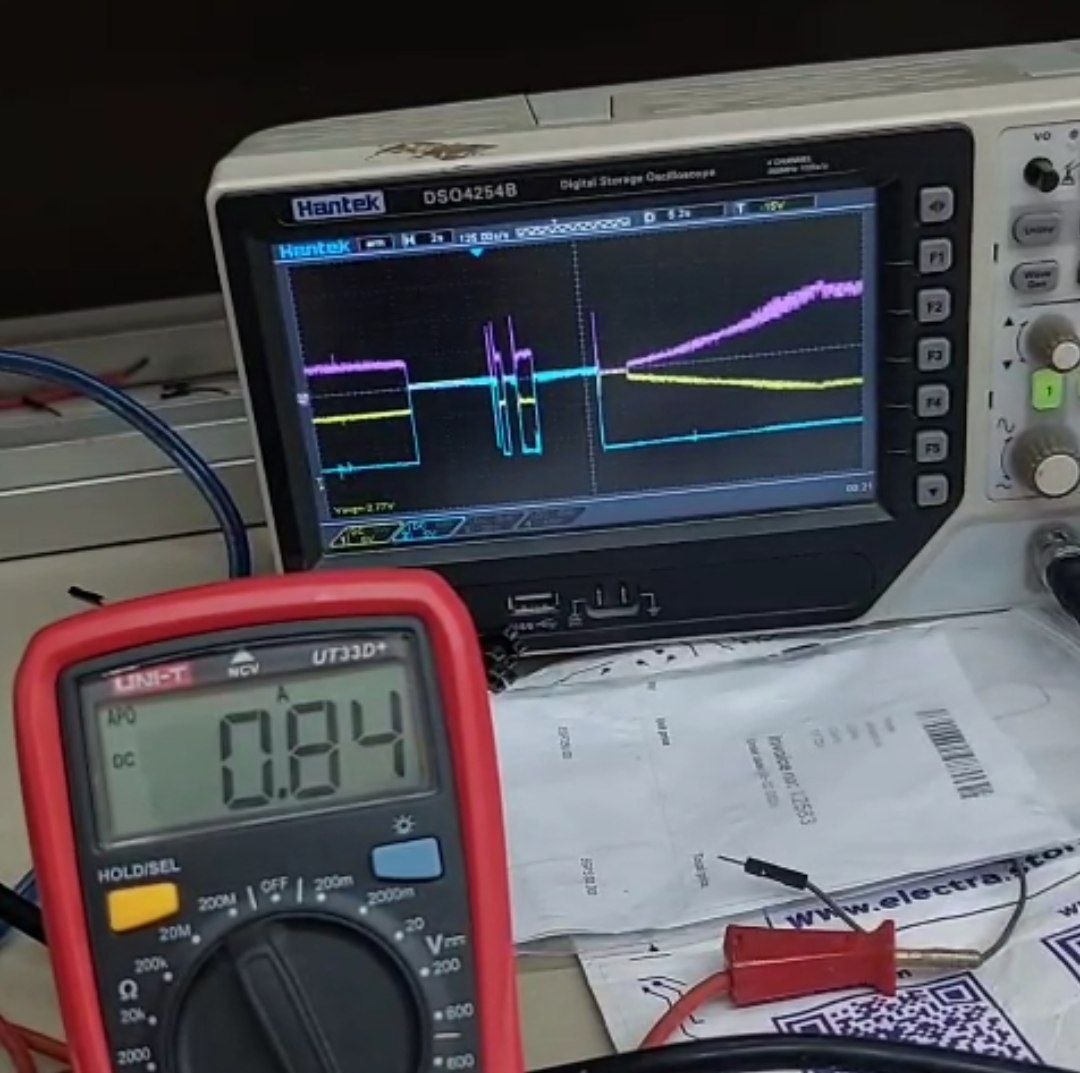
\includegraphics[width=0.85\textwidth]{Figures/mppt.jpg}
    \caption{Experimental hardware tracking trajectory showcasing dynamic automatic navigation and locking onto the absolute Maximum Power Point (MPP).}
    \label{fig:mppt_tracking_curves_auto}
\end{figure}

% =========================================================================
% SECTION: CHAPTER CONCLUSION
% =========================================================================
\subsection{Chapter Summary and Conclusion}
This chapter presented the comprehensive design, validation, and empirical verification of the generation and power conditioning stages developed for the solar-powered EV charging station infrastructure. By combining robust MATLAB/Simulink computational modeling with physical prototype hardware implementation, the structural and dynamic performance boundaries of the sub-system architectures were systematically evaluated.

The investigation successfully validated the performance metrics across three core electronic domains:
\begin{enumerate}
    \item \textbf{Interleaved Boost Input Interfacing:} Both the simulation profiles and hardware implementation verified the distinct operational advantages of the two-phase interleaved topology. Splitting the current path downscaled physical stress on passive elements, while the critical $180^\circ$ phase-shift modulation achieved destructive current ripple cancellation. This framework stabilized the input power extraction and protected the health of the primary photovoltaic source.
    \newpage
    \item \textbf{Robust Localized Intermediate Clamping:} Transitioning the central loop from linear control schemes to a dedicated closed-loop Hysteresis Voltage Regulator established an invariant intermediate bus. Hardware tests involving a high-frequency load-switching branch connected in series with a $47\ \Omega$ load resistor confirmed the controller's rapid dynamic bandwidth. The bang-bang switching logic clamped the intermediate DC-Link firmly at the target $10\text{ V}$ baseline within milliseconds of sharp transient step-load disruptions.
    \item \textbf{Automated Maximum Power Point Alignment:} To optimize source-side generation efficiency under fluctuating atmospheric conditions, a advanced hybrid optimization tracker was deployed. Manual testing across discrete duty cycle boundaries ($D = 0.50$ to $D = 0.90$) mapped the non-linear path of the physical characteristic curve. This paved the way for an autonomous embedded execution engine. The digital firmware combines a high-speed global parameter sweep with an adaptive Perturb and Observe (P\&O) tracking loop, autonomously regulating the input impedance to eliminate tracking losses and keep power injection locked at the peak efficiency vertex.
\end{enumerate}

Ultimately, the tight correlation observed between the analytical calculations, high-fidelity Simulink models, and real-world embedded firmware responses confirms the structural viability and mathematical accuracy of the converter architecture. The successful realization of this stable, high-bandwidth power processing link establishes a reliable foundation for the downstream dual-quadrant battery management storage units, satisfying the comprehensive microgrid autonomy constraints required for sustainable electric vehicle charging operations.